\documentclass[letterpaper, peerreview]{IEEEtran}
%
% If IEEEtran.cls has not been installed into the LaTeX system files,
% manually specify the path to it like:
% \documentclass[journal]{../sty/IEEEtran}

% *** CITATION PACKAGES ***
%
\usepackage{cite}
\usepackage[hidelinks]{hyperref}
% cite.sty was written by Donald Arseneau
% V1.6 and later of IEEEtran pre-defines the format of the cite.sty package
%\cite{} output to follow that of the IEEE. Loading the cite package will
% result in citation numbers being automatically sorted and properly
% 'compressed/ranged'. e.g., [1], [9], [2], [7], [5], [6] without using
% cite.sty will become [1], [2], [5]--[7], [9] using cite.sty. cite.sty's
%\cite will automatically add leading space, if needed. Use cite.sty's
% noadjust option (cite.sty V3.8 and later) if you want to turn this off
% such as if a citation ever needs to be enclosed in parenthesis.
% cite.sty is already installed on most LaTeX systems. Be sure and use
% version 5.0 (2009-03-20) and later if using hyperref.sty.
% The latest version can be obtained at:
% http://www.ctan.org/pkg/cite
% The documentation is contained in the cite.sty file itself.

% *** GRAPHICS RELATED PACKAGES ***
%
\ifCLASSINFOpdf{}
  \usepackage[pdftex]{graphicx}
  % declare the path(s) where your graphic files are
  \graphicspath{{./pdf/}{./jpg/}}
  % and their extensions so you won't have to specify these with
  % every instance of \includegraphics
  \DeclareGraphicsExtensions{.pdf,.jpg,.png}
\else
  % or other class option (dvipsone, dvipdf, if not using dvips). graphicx
  % will default to the driver specified in the system graphics.cfg if no
  % driver is specified.
  % \usepackage[dvips]{graphicx}
  % declare the path(s) where your graphic files are
  % \graphicspath{{../eps/}}
  % and their extensions so you won't have to specify these with
  % every instance of \includegraphics
  % \DeclareGraphicsExtensions{.eps}
\fi

% *** MATH PACKAGES ***
%
\usepackage{amsmath}
\newcommand*\mean[1]{\bar{#1}}
% A popular package from the American Mathematical Society that provides
% many useful and powerful commands for dealing with mathematics.

% *** SPECIALIZED LIST PACKAGES ***

% *** ALIGNMENT PACKAGES ***
%
%\usepackage{array}
% Frank Mittelbach's and David Carlisle's array.sty patches and improves
% the standard LaTeX2e array and tabular environments to provide better
% appearance and additional user controls. As the default LaTeX2e table
% generation code is lacking to the point of almost being broken with
% respect to the quality of the end results, all users are strongly
% advised to use an enhanced (at the very least that provided by array.sty)
% set of table tools. array.sty is already installed on most systems. The
% latest version and documentation can be obtained at:
% http://www.ctan.org/pkg/array

% IEEEtran contains the IEEEeqnarray family of commands that can be used to
% generate multiline equations as well as matrices, tables, etc., of high
% quality.

% *** SUBFIGURE PACKAGES ***
\ifCLASSOPTIONcompsoc
 \usepackage[caption=false,font=normalsize,labelfont=sf,textfont=sf]{subfig}
\else
 \usepackage[caption=false,font=footnotesize]{subfig}
\fi
% subfig.sty, written by Steven Douglas Cochran, is the modern replacement
% for subfigure.sty, the latter of which is no longer maintained and is
% incompatible with some LaTeX packages including fixltx2e. However,
% subfig.sty requires and automatically loads Axel Sommerfeldt's caption.sty
% which will override IEEEtran.cls' handling of captions and this will result
% in non-IEEE style figure/table captions. To prevent this problem, be sure
% and invoke subfig.sty's 'caption=false' package option (available since
% subfig.sty version 1.3, 2005/06/28) as this is will preserve IEEEtran.cls
% handling of captions.
% Note that the Computer Society format requires a larger sans serif font
% than the serif footnote size font used in traditional IEEE formatting
% and thus the need to invoke different subfig.sty package options depending
% on whether compsoc mode has been enabled.

% *** FLOAT PACKAGES ***
%
%\usepackage{fixltx2e}
% fixltx2e, the successor to the earlier fix2col.sty, was written by
% Frank Mittelbach and David Carlisle. This package corrects a few problems
% in the LaTeX2e kernel, the most notable of which is that in current
% LaTeX2e releases, the ordering of single and double column floats is not
% guaranteed to be preserved. Thus, an unpatched LaTeX2e can allow a
% single column figure to be placed prior to an earlier double column
% figure.
% Be aware that LaTeX2e kernels dated 2015 and later have fixltx2e.sty's
% corrections already built into the system in which case a warning will
% be issued if an attempt is made to load fixltx2e.sty as it is no longer
% needed.
% The latest version and documentation can be found at:
% http://www.ctan.org/pkg/fixltx2e

%\usepackage{stfloats}
% stfloats.sty was written by Sigitas Tolusis. This package gives LaTeX2e
% the ability to do double column floats at the bottom of the page as well
% as the top. (e.g., '\begin{figure*}[!b]' is not normally possible in
% LaTeX2e). It also provides a command:
%\fnbelowfloat
% to enable the placement of footnotes below bottom floats (the standard
% LaTeX2e kernel puts them above bottom floats). This is an invasive package
% which rewrites many portions of the LaTeX2e float routines. It may not work
% with other packages that modify the LaTeX2e float routines. The latest
% version and documentation can be obtained at:
% http://www.ctan.org/pkg/stfloats
% Do not use the stfloats baselinefloat ability as the IEEE does not allow
% \baselineskip to stretch. Authors submitting work to the IEEE should note
% that the IEEE rarely uses double column equations and that authors should try
% to avoid such use. Do not be tempted to use the cuted.sty or midfloat.sty
% packages (also by Sigitas Tolusis) as the IEEE does not format its papers in
% such ways.
% Do not attempt to use stfloats with fixltx2e as they are incompatible.
% Instead, use Morten Hogholm'a dblfloatfix which combines the features
% of both fixltx2e and stfloats:
%
% \usepackage{dblfloatfix}
% The latest version can be found at:
% http://www.ctan.org/pkg/dblfloatfix

% *** PDF, URL AND HYPERLINK PACKAGES ***
%
\usepackage{url}
% url.sty was written by Donald Arseneau. It provides better support for
% handling and breaking URLs. url.sty is already installed on most LaTeX
% systems. The latest version and documentation can be obtained at:

% correct bad hyphenation here
\hyphenation{op-tical net-works semi-conduc-tor}

\usepackage[nolist]{acronym}

\usepackage{booktabs}
\usepackage{adjustbox}

\usepackage[utf8]{inputenc}
% enables custom font styles which are not available in IEEEtrans by default
% https://tex.stackexchange.com/questions/331228/there-is-no-bold-text-italics-in-ieeetran

\renewcommand{\sfdefault}{cmss}
\renewcommand{\rmdefault}{cmr}
\renewcommand{\ttdefault}{cmt}

\usepackage[detect-all]{siunitx}

\begin{document}
%
% paper title
% Titles are generally capitalized except for words such as a, an, and, as,
% at, but, by, for, in, nor, of, on, or, the, to and up, which are usually
% not capitalized unless they are the first or last word of the title.
% Linebreaks \\ can be used within to get better formatting as desired.
% Do not put math or special symbols in the title.
\title{Supporting Ecological Decision Making Using Feature-Selection and Variable Importance}
\IEEEpeerreviewmaketitle{Supporting Ecological Decision Making Using Feature-Selection and Variable Importance}
%
%
% author names and IEEE memberships
% note positions of commas and nonbreaking spaces ( ~ ) LaTeX will not break
% a structure at a ~ so this keeps an author's name from being broken across
% two lines.
% use \thanks{} to gain access to the first footnote area
% a separate \thanks must be used for each paragraph as LaTeX2e's \thanks
% was not built to handle multiple paragraphs
%

% suppress 'underfull hbox' warnings
\hbadness=99999

\author{Patrick~Schratz,~\IEEEmembership{Member,~IEEE,}
	Jannes~Muenchow,~\IEEEmembership{Member,~IEEE,}
	Eugenia Iturritxa,~\IEEEmembership{Member,~IEEE,}
	José Cortés,~\IEEEmembership{Member,~IEEE,}
	Bernd~Bischl,~\IEEEmembership{Member,~IEEE,}
	and Alexander~Brenning,~\IEEEmembership{Member,~IEEE}
	\thanks{P. Schratz, J. Muenchow, J. Cortés and A. Brenning are with the Department
		of Geography, GIScience group, Friedrich-Schiller-University of Jena, Germany.}% <-this % stops a space
	\thanks{B. Bischl is head of the computational statistics group at the Department of Statistics, Ludwig-Maximilian-University Munich.}% <-this % stops a space
	\thanks{E. Iturritxa is with NEIKER Tecnalia, Vitoria-Gasteiz, Arab, Spain.}% <-this % stops a space
	%\thanks{Manuscript received April 19, 2005; revised August 26, 2015.}
}

% note the % following the last \IEEEmembership and also \thanks -
% these prevent an unwanted space from occurring between the last author name
% and the end of the author line. i.e., if you had this:
%
% \author{....lastname \thanks{...} \thanks{...} }
%                     ^------------^------------^----Do not want these spaces!
%
% a space would be appended to the last name and could cause every name on that
% line to be shifted left slightly. This is one of those 'LaTeX things'. For
% instance, '\textbf{A} \textbf{B}' will typeset as 'A B' not 'AB'. To get
% 'AB' then you have to do: '\textbf{A}\textbf{B}'
% \thanks is no different in this regard, so shield the last } of each \thanks
% that ends a line with a % and do not let a space in before the next \thanks.
% Spaces after \IEEEmembership other than the last one are OK (and needed) as
% you are supposed to have spaces between the names. For what it is worth,
% this is a minor point as most people would not even notice if the said evil
% space somehow managed to creep in.

% The paper headers
\markboth{IEEE Transactions on Geoscience and Remote Sensing}%
{Shell \MakeLowercase{\textit{et al.}}: Bare Demo of IEEEtran.cls for IEEE Journals}
% The only time the second header will appear is for the odd numbered pages
% after the title page when using the twoside option.
%
% *** Note that you probably will NOT want to include the author's ***
% *** name in the headers of peer review papers.                   ***
% You can use \ifCLASSOPTIONpeerreview for conditional compilation here if
% you desire.

% make the title area
\maketitle

% As a general rule, do not put math, special symbols or citations
% in the abstract or keywords.
\begin{abstract}
	The abstract goes here.
\end{abstract}

% Note that keywords are not normally used for peer-review papers.
\begin{IEEEkeywords}
	hyperspectral imagery, forest health monitoring, machine learning, feature selection, model comparison, imaging spectroscopy
\end{IEEEkeywords}

% For peer review papers, you can put extra information on the cover
% page as needed:
\ifCLASSOPTIONpeerreview{}
%\begin{center} \bfseries EDICS Category: 3-BBND \end{center}
\fi

% For peer-review papers, this IEEEtran command inserts a page break and
% creates the second title. It will be ignored for other modes.
\IEEEpeerreviewmaketitle{}

\renewcommand{\IEEEiedlistdecl}{\IEEEsetlabelwidth{SONET}}
\begin{acronym}

	% geringerer Zeilenabstand
	
	%\setlength{\itemsep}{-\parsep}
	
	\acro{AGB}{above-ground biomass}
	\acro{ALE}{accumulated local effects}
	\acro{ALS}{airborn laser scanning}
	\acro{ANN}{artificial neural network}
	\acro{AUROC}{area under the receiver operating characteristics curve}
	\acro{BRT}{boosted regression trees}
	\acro{CART}{classification and regression trees}
	\acro{CNN}{convolutional neural networks}
	\acro{CV}{cross-validation}
	\acro{DAP}{digital aerial photogrammetry}
	\acro{ENM}{environmental niche modeling}
	\acro{FPR}{false positive rate}
	\acro{FFS}{forward feature-selection}
	\acro{FS}{feature-selection}
	\acro{GAM}{generalized additive model}
	\acro{GBM}{gradient boosting machine}
	\acro{GLM}{generalized linear model}
	\acro{ICGC}{Institut Cartografic I Geologic de Catalunya}
	\acro{IQR}{interquartile range}
	\acro{MARS}{multivariate adaptive regression splines}
	\acro{MBO}{model-based optimization}
	\acro{MEM}{maximum entropy model}
	\acro{ML}{machine learning}
	\acro{NDII}{normalized difference infrared index}
	\acro{NIR}{near-infrared}
	\acro{NRI}{normalized ratio index}
	\acro{OLS}{ordinary least squares}
	\acro{LiDAR}{light detection and ranging}
	\acro{LOWESS}{locally weighted scatter plot smoothing}
	\acro{PISR}{potential incoming solar radiation}
	\acro{PCA}{principal component analysis}
	\acro{PDP}{partial dependence plots}
	\acro{PLS}{partial least-squares}
	\acro{RBF}{radial basis function}
	\acro{RF}{random forest}
	\acro{RMSE}{root mean square error}
	\acro{RR}{ridge regression}
	\acro{RSS}{residual sum of squares}
	\acro{SAR}{synthetic aperture radar}
	\acro{SDM}{species distribution modeling}
	\acro{SMBO}{sequential-based model optimization}
	\acro{SVM}{support vector machine}
	\acro{TPR}{true positive rate}
	\acro{VI}{vegetation index}
	\acro{XGBOOST}{extreme gradient boosting}
\end{acronym}
\renewcommand{\IEEEiedlistdecl}{\relax}% reset back

\section{Introduction}
% Explain how remote sensing is used in forestry (potential to map forest health)

% Link remote sensing and machine-learning

\IEEEPARstart{T}{he} use of \ac{ML} algorithms for analyzing remote sensing data has seen a huge increase in the last decade~\cite{lary2016}.
This goes in line with the increased availability of remote sensing imagery, especially since the launch of the first Sentinel satellite in the year 2014.
At the same time, the implementation and usability of learning algorithms has been greatly simplified with many contributions from open-source efforts.
Scientists can nowadays relatively easily process large amounts of (environmental) information using various learning algorithms.
This makes it possible to extend the matrix of possible options in a semi-automated way, possibly stumbling across unexpected findings of process settings that would have never been tested otherwise~\cite{ma2015}.

% link to forest health analysis and show exemplary studies

Machine learning methods in combination with remote sensing data are used in many environmental fields such as vegetation cover analysis or forest carbon storage mapping\cite{mascaro2014, urban2018}.
The ability of predicting to large unknown areas qualifies these tools as a promising toolset for such tasks.
One aspect of this research field is to enhance the understanding of biotic and abiotic triggers, for example by analyzing defoliation at trees\cite{hawrylo2018}.

Other approaches for analyzing forest health include temporal change detection\cite{zhang2016} or describing the current health status of forests on a stand level\cite{townsend2012}.
In such studies, the defoliation of trees serves as a proxy for forest health by describing the impact of biotic and abiotic pest triggers\cite{townsend2012, goodbody2018}.

Vegetation indices have shown the potential to provide valuable information when analyzing forest health\cite{jiang2014, adamczyk2015}.
Most vegetation indices were developed with the aim of being sensitive to changes of specific wavelength regions, serving as a proxy for underlying plant processes. 
However, often enough indices developed for different purposes than the one to be analyzed can help explaining complex relationships.
This emphasizes the need to extract as much information as possible from the available input data to generate promising features which can help understanding the modeled relationship.
A less known index type which can be derived from spectral information is called normalized ratio index (NRI).
In contrast to \ac{VI}, \ac{NRI}s are not based on an expert-based formulas following environmental heuristics but use a data-driven feature engineering approach by combining (arbitrary) combinations of spectral bands.
Especially when working with hyperspectral data, hundreds of \ac{NRI} features can be derived this way.

% now that we introduced the importance of remote sensing indices for forest health,

Despite its popularity in environmental modeling, there are no studies so far which used machine learning algorithms in combination with remote sensing data to analyze defoliation on a tree level.
This study aims to close this gap by analyzing defoliation at trees in northern Spain using airborne hyperspectral data.
We make use of the latest state-of-the-art methodology in machine learning by combining feature-selection and hyperparameter tuning across multiple algorithms.
Incorporating the idea of creating data-driven \ac{NRI}s, this study also discusses the practical problems of high-dimensionality in environmental modeling \cite{trunk1979, xu2016}.

Even though \ac{ML} algorithms are capable of handling highly-correlated input variables, the fitting time of models increase substantially and the interpretation of results becomes more complicated.
At the same time, one has to deal with the presence of spatial autocorrelation in the data.
The dataset used in this study comes with a spatial grouping at the plot level which needs to be accounted for.

The research questions of this study are the following:

\begin{itemize}

	\item Do different environmental feature sets show differences in performance when modeling defoliation at trees?
	      
	\item Does combining feature sets have an substantial effect on predictive performance?
	      
	\item How are feature-selection methods influencing the predictive performance of the models?
	      
	\item Which features are most important for the models and how can these be interpreted in an ecological context?
	      
\end{itemize}

\noindent \ac{RF}, \ac{SVM} and extreme gradient boosting were fitted on six feature sets using different feature selection methods.
Bayesian Optimization, also known as model-based optimization, was used for hyperparameter tuning and optimization of the number of features.
By merging all optimization steps into a single step, multiple optimization stages, which may introduce bias cause long model fitting times, were avoided.
A spatial \ac{CV} approach on the plot level was used to account for spatial autocorrelation in the data.

\section{Data and study area}

\noindent Airborne hyperspectral data with a spatial resolution of one meter and 126 spectral bands was available for four Monterey Pine (\textit{Pinus radiata}) plantations in northern Spain.
The trees in the study area plots suffer from infections of invasive pathogens such as \textit{Diplodia sapinea}, \textit{Fusarium circinatum}, \textit{Armillaria mellea} or \textit{Heterobasidion annosum}, leading to a spread of cankers or defoliation~\cite{mesanza2016, iturritxa2017}.
In-situ measurements of defoliation at trees (serving as a proxy for tree health) were collected to serve as the response variable \textit{defoliation} which ranges from 0\% - 100\% (\autoref{fig:defol-distr}). % chktex 8
The fungi are assumed to infect the trees through open wounds, possibly caused by previous hail damage \cite{iturritxa2014}.
The dieback of these trees, which are mainly used as timber, causes high economic damages \cite{ganley2009}.

\begin{figure} [t!]
	\centering
	\begin{center}
		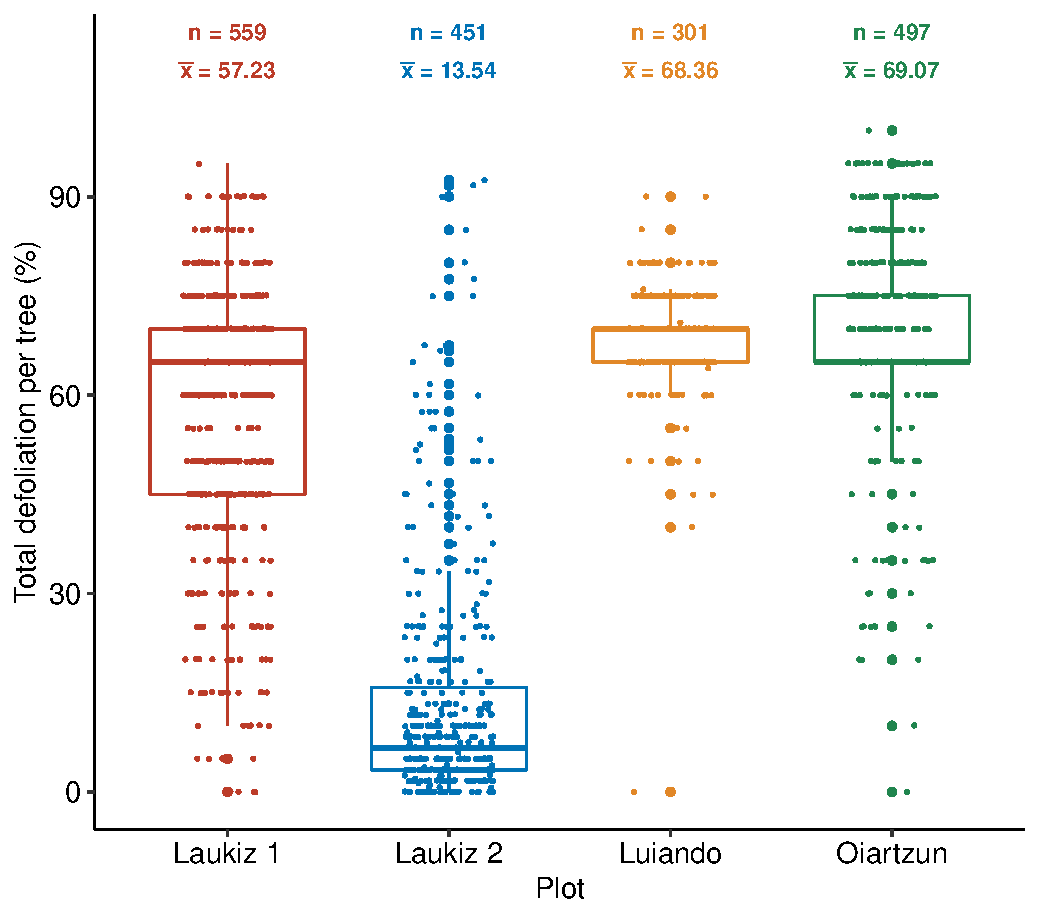
\includegraphics[width=0.48\textwidth] {defoliation-distribution-plot-1.pdf}
		\caption{Response variable \textit{defoliation} at trees for plots \textit{Laukiz 1}, \textit{Laukiz 2}, \textit{Luiando} and \textit{Oiartzun}. \texttt{n} corresponds to the total number of trees in the plot, $\bar{x}$ refers to the mean defoliation.}\label{fig:defol-distr}
	\end{center}
\end{figure}

\subsection{In-situ data}

\noindent The \textit{Pinus radiata} plots of this study, namely \textit{Laukiz 1}, \textit{Laukiz 2}, \textit{Luiando} and \textit{Oiartzun}, are located in the northern part of the Basque Country (\autoref{fig:study_area}).
\textit{Oiartzun} has the most observations (n = 559) while \textit{Laukiz 2} shows the largest area size (1.44 ha).
All plots besides \textit{Luiando} are located nearby the coast (\autoref{fig:study_area}).
In total 1808 observations are available (\textit{Laukiz 1} = 559, \textit{Laukiz 2} = 451, \textit{Luiando} = 301, \textit{Oiartzun} = 497).
The data was surveyed in September 2016.

\begin{figure} [t!]
	\begin{center}
		\centering
		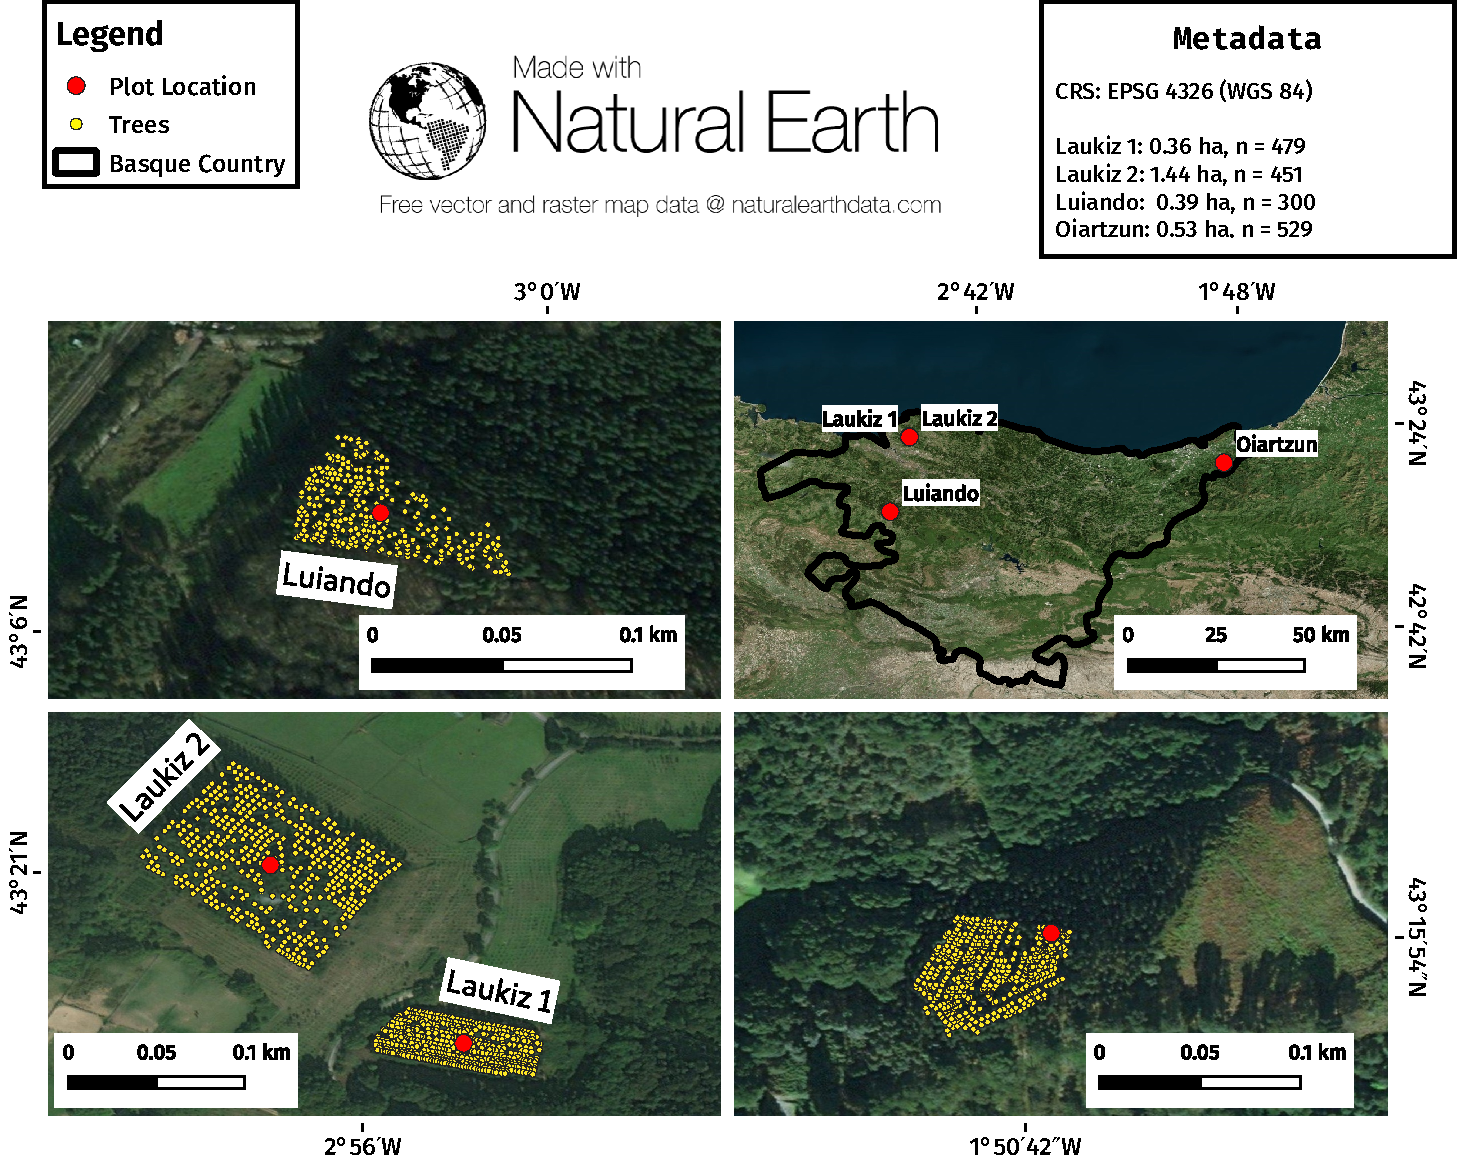
\includegraphics[width=0.48\textwidth] {study-area-hyperspectral.pdf}
		\caption{Information about location, size and spatial distribution of trees for all plots used in this study.}\label{fig:study_area}
	\end{center}
\end{figure}

%\begin{figure} [t!]
%	\begin{center}
%		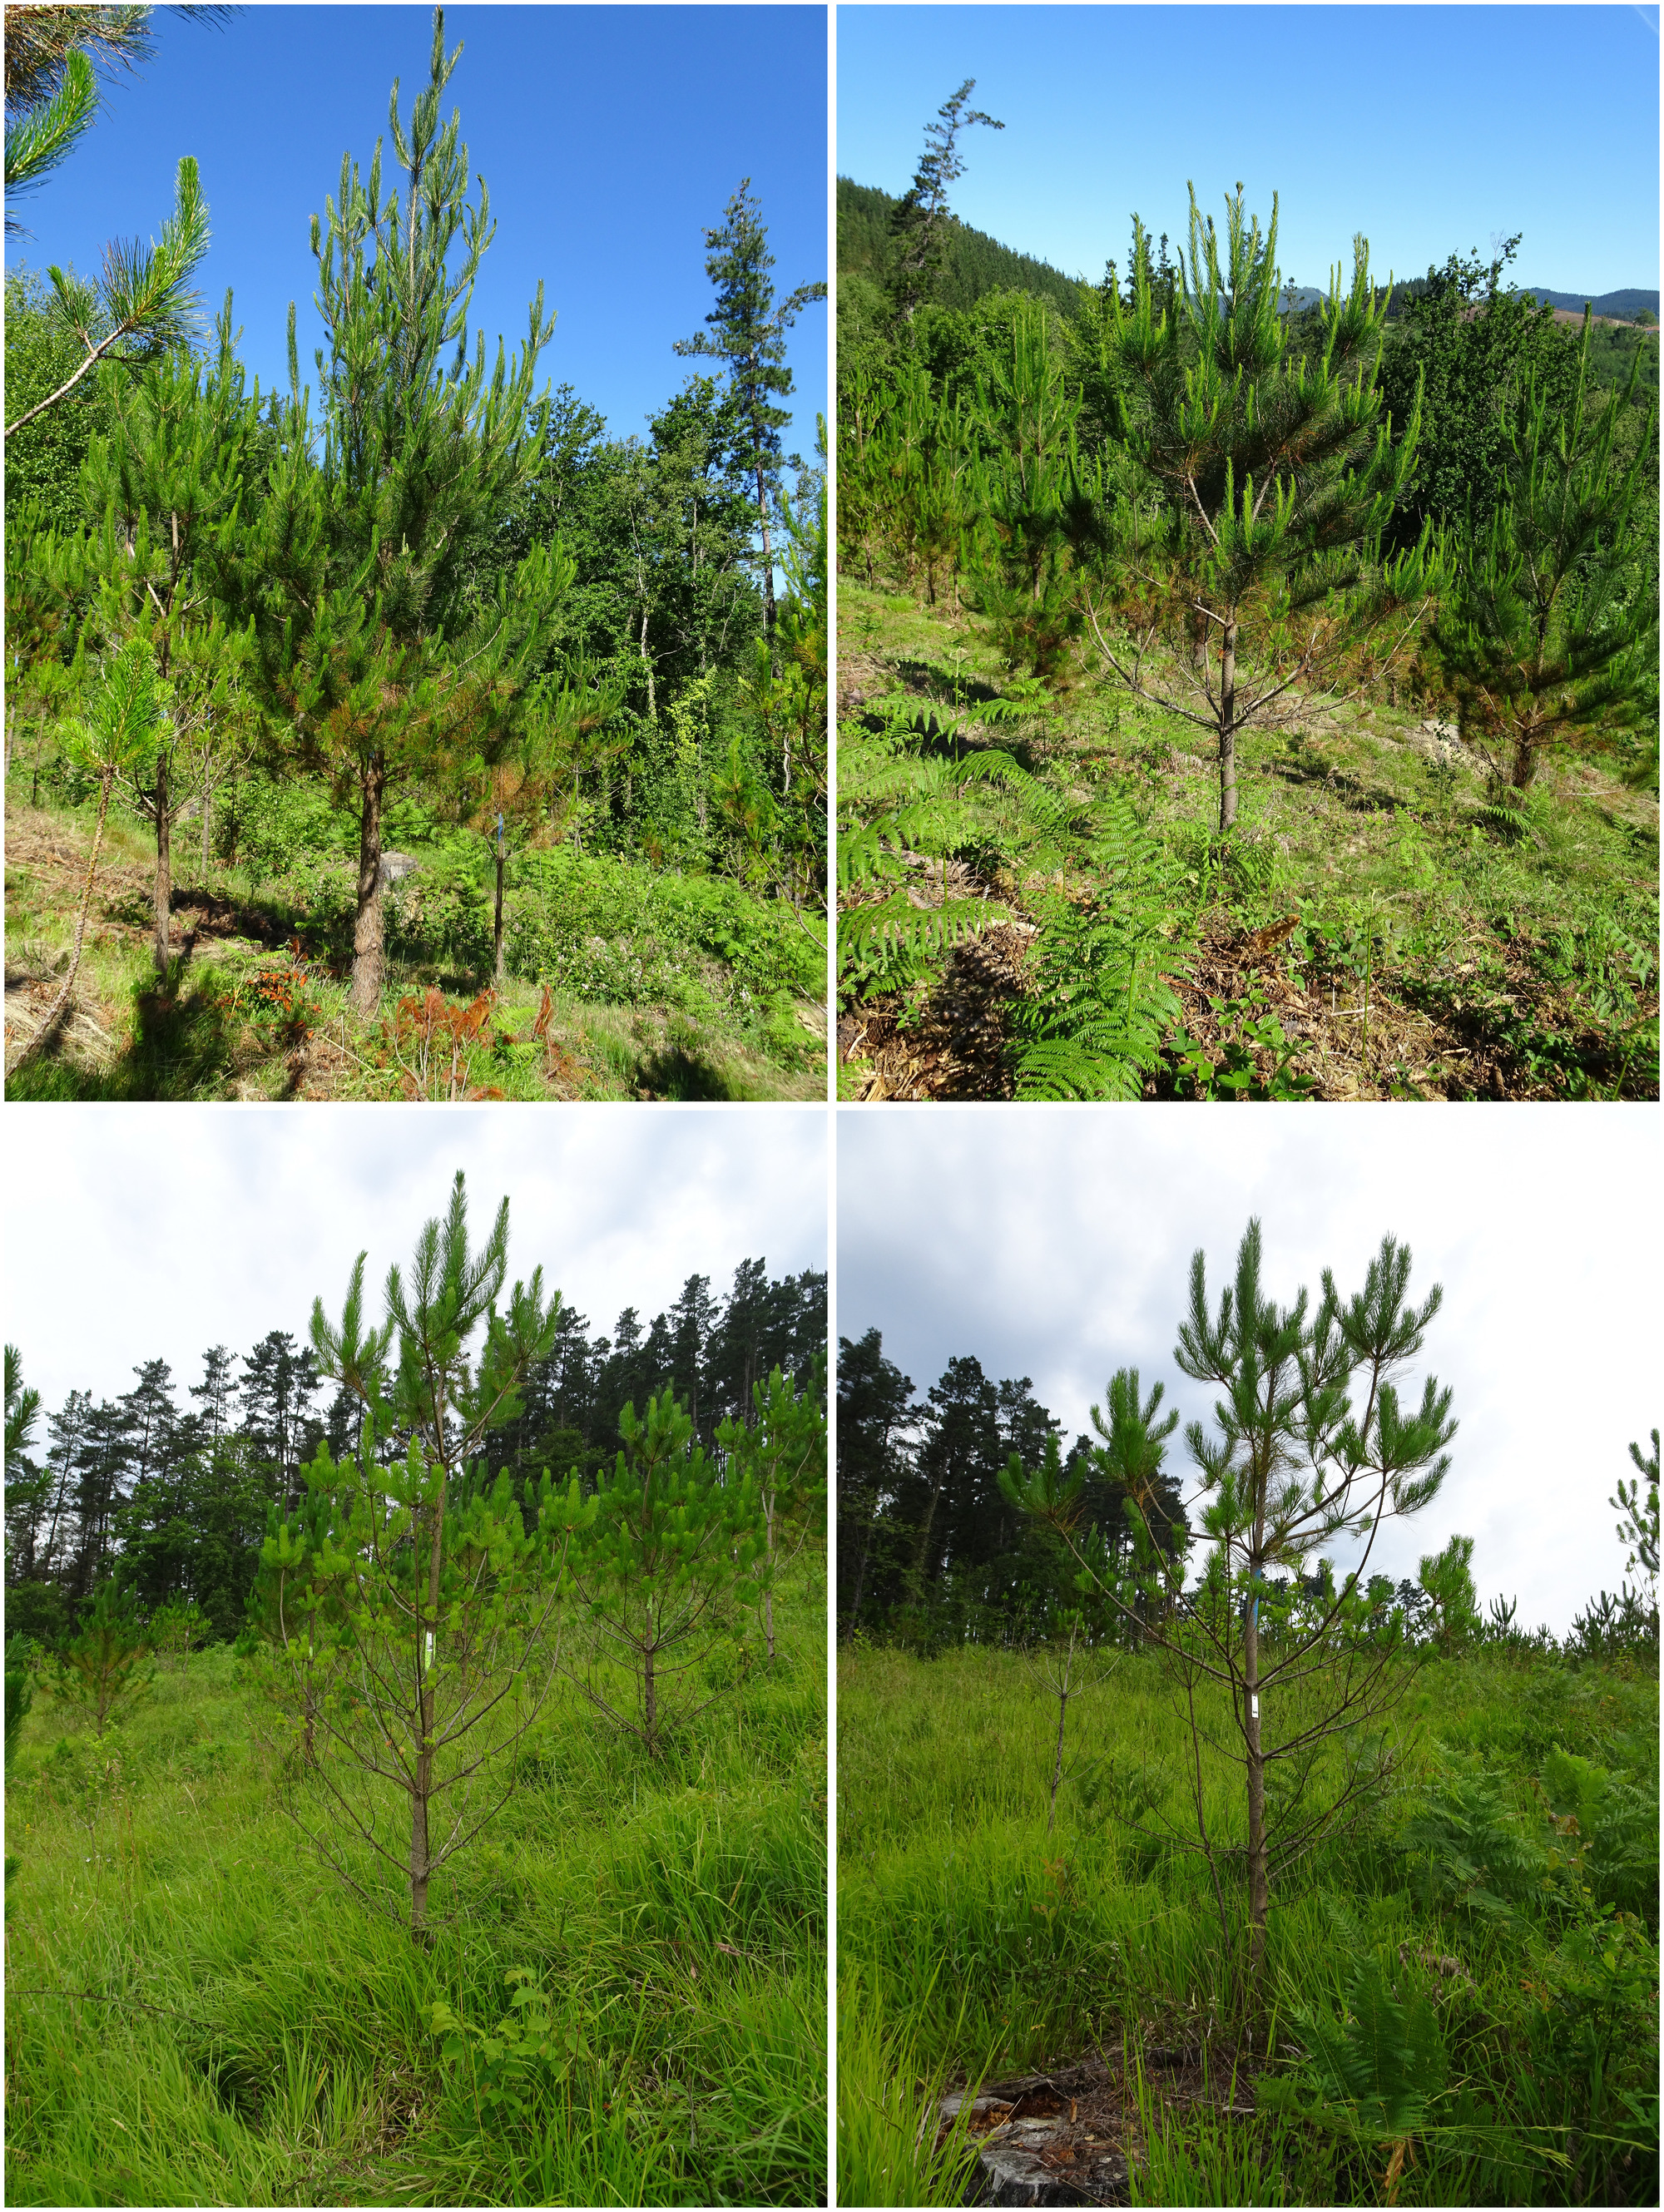
\includegraphics[width=0.48\textwidth] {defol-grid-3000px.jpg}
%		\caption{Example trees showing different levels of defoliation as interpreted by the surveyor: 10 \% (top-left), 20 \% (top-right), 40 \% (bottom-left), 60-70 \% (bottom-right).}
%		\label{fig:defol-trees}
%	\end{center}
%\end{figure}


\subsection{Hyperspectral data}

\noindent The airborne hyperspectral data was acquired during two flight campaigns on September 28th and October 5th 2016, both around 12 am.
The images were taken using a AISAEAGLE-II sensor.
All preprocessing steps (geometric, radiometric, atmospheric) have been conducted by the \ac{ICGC}.
The first four bands are corrupted, leaving 122 bands with valid information.
Additional metadata information is available in \autoref{tab:hyperparameter_limits}.

% parameter limits

\begin{table}[t]
\centering
\caption[t]{Specifications of hyperspectral data.}
\begingroup
\begin{tabular}{ll}
	\\
	Characteristic         & Value                               \\
	\toprule
	Geometric resolution   & 1 m                                 \\
	Radiometric resolution & 12 bit                              \\
	Spectral resolution    & 126 bands (404.08 nm --- 996.31 nm) \\
	Correction:            & Radiometric, geometric, atmospheric
\end{tabular}
\endgroup\label{tab:hyperparameter_limits}
\end{table}

\section{Methods}

\subsection{Derivation of indices}
\noindent To use the full potential from the hyperspectral data, all possible vegetation indices supported by the R package $\left\{hsdar\right\}$ (89 in total) as well as all possible \ac{NRI} combinations were calculated.
The following formula was used for the NRI calculation:

\begin{equation}
	NRI_{i,j} = \frac{b_{i} - b_{j}}{b_{i} + b_{j}}
\end{equation}

\noindent
where \(i\) and \(j\) are the respective band numbers.

\bigbreak{}

\noindent To account for geometric offsets (which were reported with up to 1 m from \ac{ICGC}) within the hyperspectral data, a buffer of two meters around the centroid of each tree was used during extraction of the reflectance values.
Subsequently, the value assigned to a tree observations was the mean of all pixels which were touched by the buffer drawn around each tree.
A pixel was considered to fall into a tree's buffer zone if the centroid of the respective pixel was touched by the buffer.
This is how the \texttt{extract()} function of the R package $\left\{raster\right\}$ handles buffer extraction.
In total, \(\frac{125*126}{2} = 7875\) NRIs were calculated.
Due to four corrupted bands of the sensor a total of 7471 indices were available for each observation.

\subsection{Dimension reduction}

\noindent We want to stress the differences between 'dimension reduction' and 'high-dimensionality'.
The former refers to the general idea of reducing features from a dataset \cite{vandermaaten2007}.
In modeling this means finding the best subset of covariates which provide the most predictive power to the model or extracting the main components of the features using a \ac{PCA}.
'High-dimensionality' in contrast is a dataset attribute and applies when \(p > n\), where \(p\) is the number of covariates and \(n\) the number of observations \cite{hastie2001}.
There is no absolute value at which the term applies, both for \(n\) and \(p\).
Hence for this study the word ‘high-dimensionality‘ only applies to the experiments using the ‘NRI‘ feature set ($>$ 7000 features for 1808 observations).

The case of a feature-rich dataset comes with several challenges for both model fitting and evaluation.

\begin{itemize}
	\item Model fitting times increase.
	\item Noise is possibly introduced into models by highly-correlated variables\cite{johnstoneiainm.2009}.
	\item Model interpretation and prediction tasks become more challenging\cite{johnstoneiainm.2009}.
\end{itemize}

\noindent In the following sections a brief overview about sub-categories of feature selection approaches is given.
Due to the focus of this study on the use of filter methods, which are a sub-group of feature selection methods, other approaches were grouped into a single section.

\subsubsection{Filter methods}

% Filter methods
\noindent The concept of filters originates on the idea of ranking features using certain heuristics of an algorithm \cite{chandrashekar2014}.
Some filter methods are restricted towards specific types of variables (numeric or nominal).
Filters do only rank features, they do not choose which covariates to drop or keep\cite{drotar2015}.
The selection of features to keep for the model fitting step is usually done within the optimization phase of the model fitting, along with the hyperparameter tuning.
Essentially, the number of covariates in the model is treated as a hyperparameter of the model.
The goal is to optimize the number of features (using the ranked covariates) at which the model achieves the best performance.
In well-implemented software solutions the filter calculation is only done once and then cached, saving computational resources \cite{mlr}.

\paragraph{Ensemble filter methods}

% Ensemble filter methods
Besides the concept of choosing a specific filter method to rank variables, studies showed that combining several filters using statistical operations such as 'minimum', 'mean' or 'sum' are able to enhance the predictive performance of the resulting models \cite{abeel2010, drotar2017a}.
This approach is referred to as 'ensemble filter'~\cite{dietterich2000}.
Ensemble filters align with the recent rise of the 'ensemble' approach in machine learning which uses stacking to combine the predictions of multiple models, aiming to enhance predictive performance~\cite{polikar2012, feurer2015}.
In this work the 'Borda' ensemble filter was applied~\cite{drotar2017a}.
For this filter, the final order is the sum of all single filters.

\paragraph{Ensuring a fair weighting in the ensemble}

Filter methods can be grouped into classes: Correlation based, entropy based, linear and non-linear methods.
It is important to not give certain classes too much weight in the ensemble as otherwise the final result will be biased towards these.
In this study this was taken care of by checking the rank correlations (Spearman's correlation) of the generated feature rankings of all methods against each other.
In case pairs of filters with a correlation above 0.9 were discovered, only one of these was included into the ensemble filter.
By this we ensured that the ensemble filter is not biased towards a certain group of methods yielding highly similar rankings.

\paragraph{Description of used filter methods}

Filter methods can be classified as follows:

\begin{itemize}
	\item univariate/multivariate (scoring based on a single variable / multiple variables)
	\item linear/non-linear (calculation of linear/non-linear interaction terms)
	\item entropy/correlation (scoring based on derivations of entropy or correlation based approaches)
\end{itemize}

% filter methods
\begin{table}[b!]
\centering
\caption[t]{List of filter methods used in this work}
\begingroup\footnotesize
\begin{adjustbox}{width={0.48\textwidth},totalheight={\textheight},keepaspectratio}
	\begin{tabular}{lll}
		\\
		Name                                         & Group                             & Ref.               \\
		\toprule
		Linear correlation (Pearson)                 & univariate, linear, correlation   & \cite{pearson1901} \\
		Information gain                             & univariate, non-linear, entropy   & \cite{quinlan1986} \\
		Minimum redundancy, maximum relevance        & multivariate, non-linear, entropy & \cite{zhao2013}    \\
		Carscore                                     & multivariate, linear, correlation & \cite{zuber2011}   \\
		Relief                                       & multivariate, linear, entropy,    & \cite{kira1992}    \\
		Conditional minimal information maximization & multivariate, linear, entropy     & \cite{fleuret2004}
	\end{tabular}
\end{adjustbox}
\endgroup\label{tab:filter-methods}
\end{table}

\noindent Filter 'Information Gain' is only defined for nominal response variables:

\begin{equation}
	H(Class) + H(Attribute) - H(Class, Attribute)
\end{equation}

where \(H\) is the conditional entropy of the response variable (class) or the feature (attribute), respectively.
To be able to use this method with a numeric response (defoliation in our case), the variable is discretized into equal bins and treated as a class variable.
While the number of bins can be treated as a hyperparameter of the filter method, we decided to use \texttt{\(n_{bin}\) = 10} after rank correlations of $> 0.9$ for different bin sizes were observed in a side analysis.

\subsubsection{Wrapper methods and PCA}

\noindent Other approaches to assess feature importance are so called 'wrapper methods' and the \ac{PCA}\cite{das2001, jolliffe2016}.

% Wrapper approach
\noindent Wrappers \cite{chandrashekar2014, kohavi1997} apply algorithms that are also used for hyperparameter optimization such as 'Random Search' or 'Generic Simulated Annealing'.
First a (random) subset of features is chosen based on the selected algorithm.
In comparison to filters, no ranking is done in this step.
Now the model is fitted on the data and the performance is evaluated.
This is done multiple times, depending on the defined stopping criteria set by the user (performance, runtime, evaluations).
A disadvantage of this approach is that hyperparameter tuning can only be applied after the feature-selection optimization finished.
Hence, the 'wrapper approach' is an expensive optimization method because two stages need to be run in sequential order.
Due to their extensive runtimes, wrappers were not considered in this work.

% PCA
A method with a completely different approach compared to filters and wrappers is the \ac{PCA}\cite{pearson1901, jolliffe2016}.
Here, the main components of the feature space are extracted and combined.
Most often the first two extracted main components are used since these contain the major information of the covariates.
By using the (automatically estimated) explained variance of the main components, the model can rely on a few features containing the majority of information available in the data.
This enables cheap model fitting with balanced loss of predictor information.
The disadvantage of this methodology is the lack of interpretability because the main components cannot be related back to the original covariates.

\subsection{Benchmarking design}

\subsubsection{Algorithms}

\noindent The benchmarking matrix of this study consists of the following algorithms:

\begin{itemize}
	\item  Extreme Gradient Boosting (XGBOOST)
	\item  Random Forest (RF)
	\item  Penalized Regression (both L1 (Lasso) and L2 (Ridge))
	\item  Support Vector Machine (SVM)
\end{itemize}

\noindent \ac{RF} and {SVM} are well established algorithms that are widely used in environmental modeling.
\ac{XGBOOST} (commonly abbreviated as XGBOOST) showed promising results in benchmark competitions in recent years.
Penalized regression is a statistical modeling technique capable of dealing with highly-correlated covariates by applying a penalization term which shrinks the coefficients of the model\cite{hastie2001}.
Common penalties are 'lasso' (L1) and 'ridge' (L2).
The former does not allow the full removal of variables from the model (penalization to zero) while the latter does.
Both penalties can also be combined.
The combined approach is called 'elastic net' but was not used in this work.

\subsubsection{Feature sets}
% TODO: talk about the reasons behind different features sets: environmental implications

\noindent Three feature sets were used in this study with each representing a different way of feature engineering:

\begin{itemize}
	\item The raw hyperspectral band information (HR): No feature engineering) %chktex 13
	\item Vegetation Indices (\ac{VI}): Expert-based feature engineering)
	\item Normalized Ratio Indices (\ac{NRI}): Data-driven feature engineering)
\end{itemize}

The idea of splitting the features into different sets originated from the question whether feature engineered indices from reflectance values have a positive effect on model performance.
Benchmarking all models on these distinct groups of features makes it easier to draw conclusions on their impact when keeping all other variables such as model type, tuning strategy and partitioning method constant.
However, rather than only looking at these three groups we decided to also take their combinations into account for the overall comparison:

\begin{itemize}
	\item HR + VI %chktex 13
	\item HR + NRI
	\item HR + VI + NRI
\end{itemize}

Even though the feature selection task was handed over to the filter methods in this study, we ensured to not include features with a pair-wise correlation of 1.
Having such can cause undesired effects during model fitting and feature importance calculation.
To account for such, all pair-wise correlations between features were calculated.
For pairs which exceeded the threshold of 0.9999999999 the one with the largest mean absolute correlation was removed.
This process was repeated $p$ times, each time calculating a new correlation matrix.

This preprocessing step resulted in the following final number of predictors: HR (122), VI (86), NRI (7467).

\subsubsection{Hyperparameter Optimization}

\noindent An exhaustive hyperparameter tuning was applied during nested spatial \ac{CV} for all algorithms.
Model-based Optimization \cite{mlrmbo} (MBO) was used for hyperparameter optimization.
This approach first composes \textit{n} randomly chosen hyperparameter settings out of a user defined search space.
After these \textit{n} tries have been evaluated, a new hyperparameter setting, going to be evaluated next, is proposed by a fitted surrogate model (by default a kriging method).
This strategy continues until a termination criterion, defined by the user, is reached \cite{hutter2011, jones1998}.

An initial design of 30 randomly composed hyperparameter settings and a termination criterion of 70 iterations was used, resulting in a total budget of 100 evaluated hyperparameter settings per fold.
The advantage of this tuning approach is the substantial reduction of the tuning budget required to find a setting which is close to the global minimum.
\ac{MBO} shines when being compared to methods that do not use information from previous runs, such as random search or grid search \cite{bergstra2012}.

For the filter methods, the percentage of features was added to the models as a hyperparameter.
For \ac{PCA}, the number of main components was tuned instead.
Random Forest hyperparameter \texttt{\(m_{try}\)} was modified into power transformed version \(p^{m_{try}}\) (ranging from 1 to $p$) to work on relative values of the respective datasets feature count.
Here \(p\) is the number of features of the dataset.
This was necessary to ensure that \texttt{\(m_{try}\)} was not chosen out of bounds during tuning with respect to the datasets feature count.
After the filtering, only a subset of features of the task is used for optimizing the models hyperparameters.
The size of this subset is always different since the number of features is also optimized.
Hence, the value of \texttt{\(m_{try}\)} needs to be created dynamically based on the datasets feature count.

\subsubsection{Spatial resampling}

\noindent A spatial nested cross-validation on the plot level was chosen to reduce the influence of spatial autocorrelation as much as possible \cite{schratz2019, sperrorest}.
Each plot served as one fold within the cross-validation setting, resulting in four iterations total.
For the inner level (hyperparameter tuning), \(y - 1\) folds were used (with \(y\) being the number of plots).

In total the benchmarking matrix consisted of 156 experiments (6 feature sets * 3 ML algorithms * 8 feature-selection methods + 2 * 6 L1 and L2 models).

\subsection{Feature importance estimation}

% FIXME Talk about the bias of permutation FI in highly correlated settings
\noindent Estimating feature importance for highly-correlated datasets is a complicated task.
The correlation between covariates makes it challenging to calculate an unbiased estimate for single features.
Methods like \ac{PDP} do not produce reliable estimates in such scenarios because unrealistic situations between covariates are created \cite{molnar2019}.
% FIXME: Add ref
Due to the noisiness of the dataset, estimates from model-agnostic approaches such as permutation-based feature importance should also be taken with care.
This method calculates the loss of predictive performance for each feature by permuting it in a random manner.
The more important the feature is for the model, the higher the variance in the measure, reflecting the importance of the specific feature for the current model.
Permuting every feature $y$ times comes with some computational cost.
To balance the effort/gain ratio and cope with limited visual space in plots, we estimated the feature importance only for datasets HR and VI using the best performing learner of the benchmark.

However, as of today there are no unbiased approaches for estimating feature importance for (highly-) correlated datasets.
Nevertheless, recent methods like \ac{ALE} plots aim to tackle this problem by utilizing marginal distributions of features over a small window to focus on the effect of a single feature \cite{apley2019, molnar2019}.
However, ALE plots need visual inspection and as the number of features increases, making objective comparisons becomes more complicated.

In this work we applied permutation-based feature importance and \ac{ALE} plots to calculate feature importance for the HR dataset.
With the limitations of both methods in mind we aimed to get a general overview of the feature importance of the hyperspectral bands while keeping modest on over-interpreting the results.
We used the algorithm which showed the best performance for the HR (SVM) task to calculate the feature importance.
ALE plots were not discussed in greater detail and are available as supplementary material.

\subsection{Linking feature importance to wavelength regions}

\noindent For ecological interpretation purposes we linked the ten most important indices of the winning models for each feature set to the spectral regions of the hyperspectral data.
For feature set HR and NRI a direct linking to the respective bands of the hyperspectral sensor was done.
For the vegetation indices all bands covered by the spectral range of calculated vegetation indices were counted and summed up.

\subsection{Research compendium}

\noindent The complete study was done using the open-source statistical programming language R \cite{rcoreteam2019}.
All R packages used in this study can be found in linked repositories.
Due to space limitations we will only mention the packages of the used algorithms and filter methods.

The algorithm implementations of the following packages have been used: \textit{xgboost}\cite{chen2016} (\textit{xgboost}), \textit{kernlab}\cite{kernlab} (Support Vector Machine) and \textit{glmnet}\cite{glmnet} (Ridge Regression).
The filter implementations of the following packages have been used: \textit{praznik\cite{praznik}}, \textit{FSelectorRcpp}\cite{fselectorrcpp}.
The R package \textit{mlr} \cite{mlr} was used for all modeling related steps.
\textit{drake} \cite{drake} was used for structuring the work and reproducibility.
This study is available as a research compendium on Zenodo (\url{10.5281/zenodo.2635403}).
The code base is available on GitHub (\url{https://github.com/pat-s/2019-feature-selection}).

\section{Results}

\subsection{Predictive performance}

% - RMSE around 27
% - MBO tuned penalized methods are substantially worse
\noindent Overall, the response variable 'defoliation at trees' could be modeled with an error of 28 \%.
SVM showed no differences in RMSE across feature sets whereas other learners like RF differed up to seven percentage points (HR-NRI vs. VI) (\autoref{fig:perf-result}).
Ridge and Lasso faced major issues up to the point of not achieving an error below 50 for datasets HR-NRI-VI and NRI-VI.
SVM showed the best performance of all learners with an absolute difference up around three percentage points to the next model (RF) (\autoref{tab:best-learner-perf}).
A high intra-fold variance was observed: Predicting on Luiando resulted in an RMSE value of 9.0 for learner SVM (without filter) but up to 54.26 RMSE when testing on Laukiz2 (\autoref{tab:svm-single-fold-perf}).

% tasks
% - no substantial difference between feature sets
% - combining feature sets has only small impact
% - expert based feature sets show no better result than data-driven ones
% - penalized methods seem to have problems with VI feature set
The combination of feature sets showed small increases in performance for some learners.
RF and XGBoost scored slightly better on the combined datasets HR-NRI and NRI-VI, respectively (\autoref{fig:perf-result}).
Datasets containing derived features (VI, NRI) showed no improvement in performance compared to the raw hyperspectral band information (HR).
All learners besides SVM show a substantially worse performance on the VI dataset (around five percentage points).

% learner
% - SVM Car is the overall winner
% - Ridge-CV hit and miss (hit = NRI, miss = VI)
% - all MBO penalized methods have no difference across tasks
SVM combined with the 'Carscore' filter achieved the best performance (RMSE of 27.98) (\autoref{tab:perf-top-10}).
%L1 penalized regression showed slightly better results in three out of six tasks when being optimized using the package internal 10-fold CV compared to MBO (RMSE of 50 vs 58).
Regression with Ridge penalty (L2) showed a high variance when comparing results across tasks: In two out of six tasks (all including VI variables) the error was out of bounds (HR-NRI-VI, HR-VI, VI). For HR-NRI and HR the error was around 40 RMSE, and for task NRI the Ridge learner achieved almost the same score as the best performing model (32.9 RMSE) (\autoref{tab:perf-top-10}).
In all settings for which Ridge showed such a high error, only one observation in one fold was predicted which such a high value (in the millions).
This then caused the error estimates of these folds and the average estimate across all folds to be out of bounds.

FIXME: Mention: All penalized methods tuned using MBO showed exactly the same error across all tasks.
FIXME: Mention the bad perf of RIDGE on VI

% filters
% - influence varies based on algorithm and task (SVM no influence, RF medium, XGB medium)
% - no substantial decrease in performance when using filters
% - no advantage of ensemble borda filter compared to others
Effects of filter methods on performance differed greatly between algorithms:
SVM showed no variation in performance across filters (\autoref{fig:filter-effects-no-filter}).
Using filters for RF showed a substantial increase in performance for all tasks besides VI for which the overall difference of all filters was also smallest (\autoref{fig:filter-effects-no-filter}).
XGBoost showed a high dependency on filtering the data: In 4 out of 6 tasks using no filter would results in the worst or second worst performance.
However, in contrast for dataset NRI using no filter results in the best performance.
XGBoost shows the highest overall differences between filters for a single task: For dataset HR, the range is up to 14 percentage points (Carscore vs. no filter)(\autoref{fig:filter-effects-no-filter}).

% filter vs. no filter
% - Substantial effect for XGBoost and RF
% - SVM unaffected
When comparing the usage of filters against using no filter at all, there was only one instance (XGBoost on the NRI task) when the model without filtering showed a slighly better performance than the best filtered one (\autoref{fig:filter-effects-no-filter}).
For SVM filters and no filter come in at the same performance for tasks VI and NRI even though \autoref{fig:filter-effects-no-filter} lists "No Filter" as the best option.

% Borda vs. other filters
% - most often among the first best filters for each task
% - never the best
The Borda filter did not achieve the best performance for any learner across any task \autoref{fig:filter-effects-borda}.
For RF and XGBoost it ranked within the first 50\% when looking at all filters used for a task.
For XGBoost on the VI task the Borda filter scored the second worst performance.

% latex table top 10 absolute performances
% latex table generated in R 3.6.1 by xtable 1.8-3 package
\begin{table}[ht!]
\centering
\caption{Best ten results for any task/learner/filter combination, sorted ascending by RMSE} 
\label{tab:perf-top-10}
\begin{tabular}{rlllrr}
  \hline
 & Task & Model & Filter & RMSE & SE \\ 
  \hline
1 & NRI & SVM & Info Gain & 27.99 & 19.15 \\ 
  2 & HR-NRI-VI & SVM & Relief & 28.07 & 19.14 \\ 
  3 & VI & SVM & Relief & 28.10 & 19.14 \\ 
  4 & HR-NRI-VI & SVM & Car & 28.11 & 19.13 \\ 
  5 & HR-NRI & SVM & MRMR & 28.12 & 19.11 \\ 
  6 & VI & SVM & Pearson & 28.12 & 19.10 \\ 
  7 & HR-NRI & SVM & CMIM & 28.12 & 19.09 \\ 
  8 & HR & SVM & Info Gain & 28.12 & 19.12 \\ 
  9 & HR & SVM & CMIM & 28.12 & 19.12 \\ 
  10 & NRI-VI & SVM & PCA & 28.12 & 19.12 \\ 
   \hline
\end{tabular}
\end{table}


% latex table worst 10 absolute performances
%% latex table generated in R 3.6.1 by xtable 1.8-3 package
\begin{table}[ht!]
\centering
\caption{Worst ten results among all combinations, sorted in decreasing order of RMSE} 
\label{tab:perf-worst-10}
\begin{tabular}{rlllr}
  \hline
 & Task & Model & Filter & RMSE \\ 
  \hline
1 & VI & Ridge-MBO & No Filter & 49359394487.65 \\ 
  2 & HR-NRI & Ridge-MBO & No Filter & 12650121073.66 \\ 
  3 & HR-NRI-VI & Ridge-MBO & No Filter & 12631934180.91 \\ 
  4 & NRI-VI & Ridge-MBO & No Filter & 11658468597.68 \\ 
  5 & HR & XGBoost & No Filter & 46.80 \\ 
  6 & VI & XGBoost & Car & 46.40 \\ 
  7 & VI & XGBoost & MRMR & 46.26 \\ 
  8 & VI & XGBoost & Borda & 46.04 \\ 
  9 & VI & XGBoost & No Filter & 45.69 \\ 
  10 & VI & XGBoost & Pearson & 44.61 \\ 
   \hline
\end{tabular}
\end{table}


% latex table best performance per learner
% latex table generated in R 3.6.1 by xtable 1.8-3 package
\begin{table}[ht!]
\centering
\caption{Best performance of each learner across any task and filter method.} 
\label{tab:best-learner-perf}
\scalebox{0.9}{
\begin{tabular}{rlllrr}
  \hline
 & Task & Model & Filter & RMSE & SE \\ 
  \hline
1 & NRI & SVM & Info Gain & 27.99 & 19.15 \\ 
  2 & NRI & RF & Car & 30.77 & 16.86 \\ 
  3 & VI & Lasso-MBO & No Filter & 31.01 & 14.71 \\ 
  4 & HR-NRI-VI & XGBoost & Borda & 31.05 & 17.01 \\ 
  5 & NRI & Ridge-MBO & No Filter & 31.16 & 15.03 \\ 
   \hline
\end{tabular}
}
\end{table}


% latex table top 20 absolute performances
% latex table generated in R 3.6.1 by xtable 1.8-3 package
\begin{table}[ht!]
\centering
\caption{Test fold performances for learner SVM on the HR dataset without using a filter. For each row, the model was trained on observations from all others plots but the given one and tested on the observations of the given plot.} 
\label{tab:svm-single-fold-perf}
\begin{tabular}{rrrl}
  \hline
 & Plot & RMSE & Test Plot \\ 
  \hline
1 &   1 & 21.17 & Laukiz1 \\ 
  2 &   2 & 28.05 & Oiartzun \\ 
  3 &   3 & 9.00 & Luiando \\ 
  4 &   4 & 54.26 & Laukiz2 \\ 
   \hline
\end{tabular}
\end{table}


% plot performance results
\begin{figure} [t!]
	\centering
	\begin{center}
		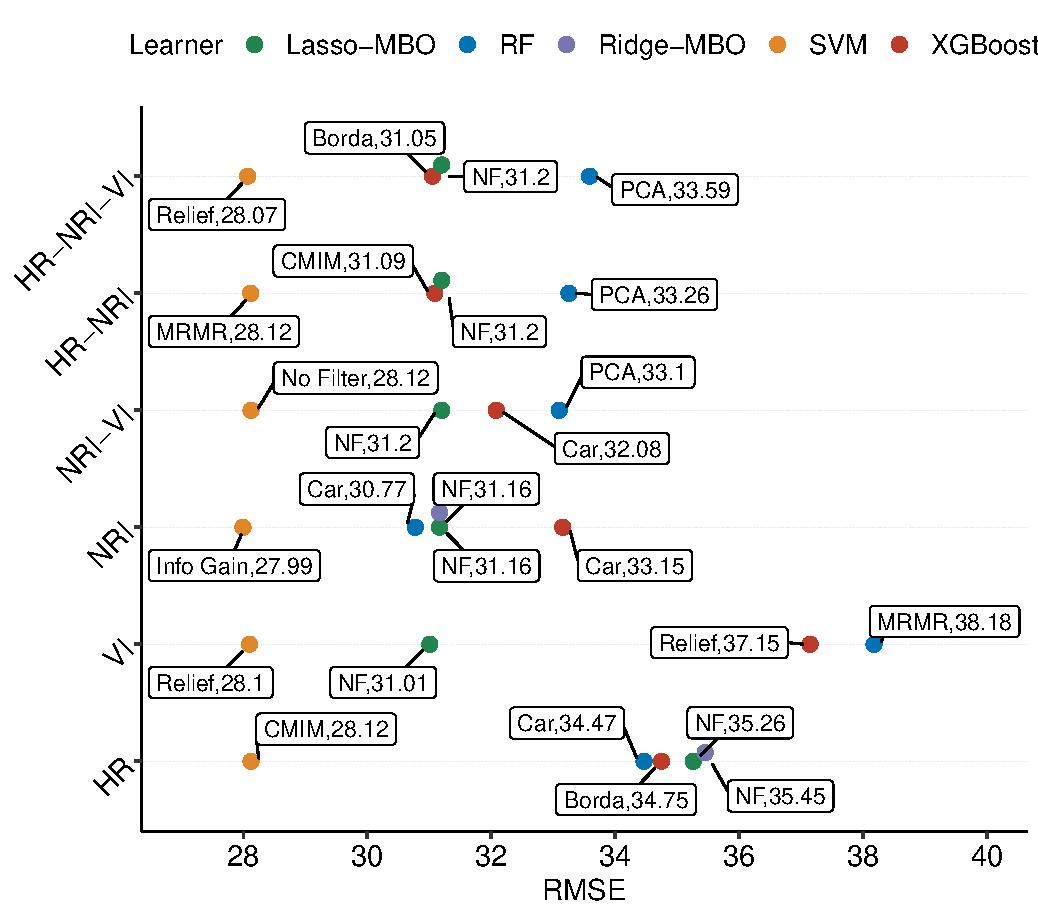
\includegraphics[width=0.48\textwidth] {performance-results-1.pdf}
		\caption{Scored predictive performance (RMSE) of models across tasks. Prefix 'CV' denotes that the learner was optimized using internal 10-fold CV while prefix 'MBO' means that Bayesian optimization was used for hyperparameter optimization. The abbreviations on the y-axis refer to the combinations of feature sets on which each model was scored on. Labels attached to each point in space show which filter method was used for scoring features during the feature selection process (NF = no filter, Car = 'Carscore', Info = 'Information Gain', Borda = 'Borda'). The second value in the attached label of each point shows the scored RMSE value of the respective setting.}\label{fig:perf-result}
	\end{center}
\end{figure}

% plot no filter vs all other filters for each model and task
\begin{figure} [t!]
	\centering
	\begin{center}
		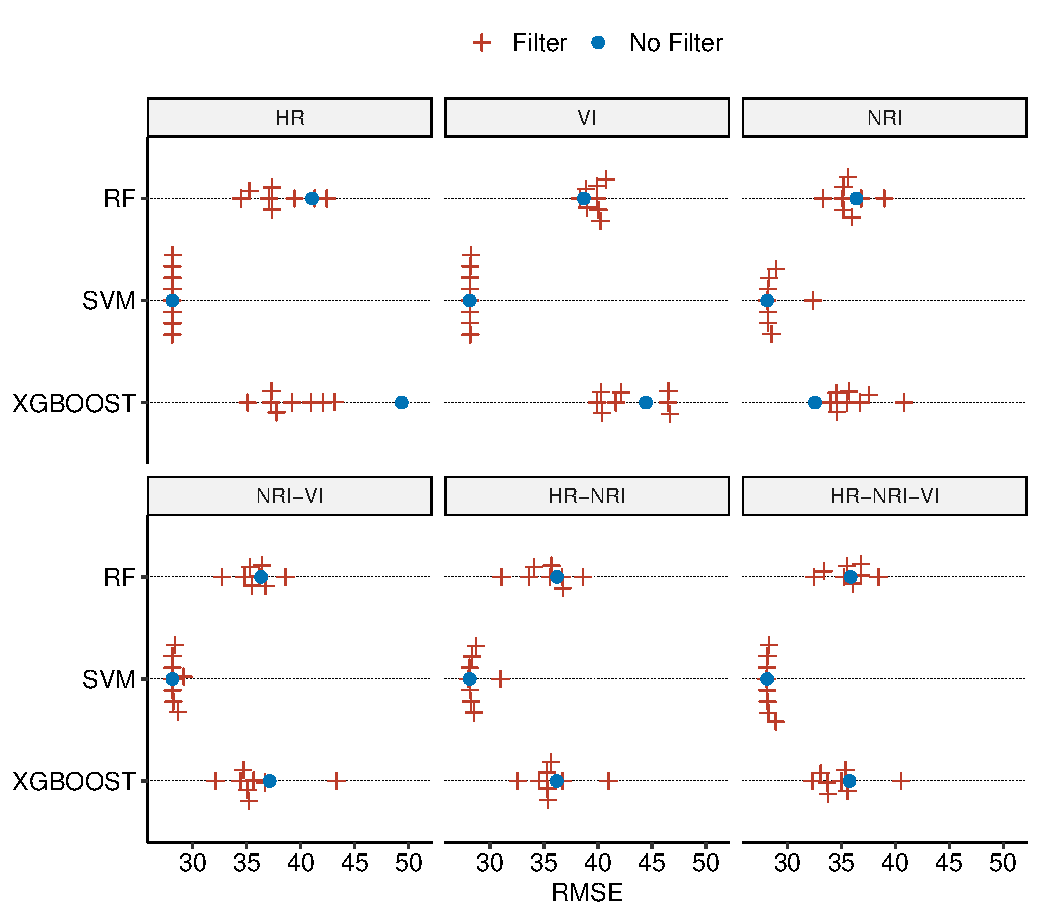
\includegraphics[width=0.48\textwidth] {filter-effect-all-vs-no-filter-1.pdf}
		\caption{Model performances in RMSE when using no filter method compared to all other filters across all tasks.}\label{fig:filter-effects-no-filter}
	\end{center}
\end{figure}

% plot Borda vs all other filters for each model and task
\begin{figure} [t!]
	\centering
	\begin{center}
		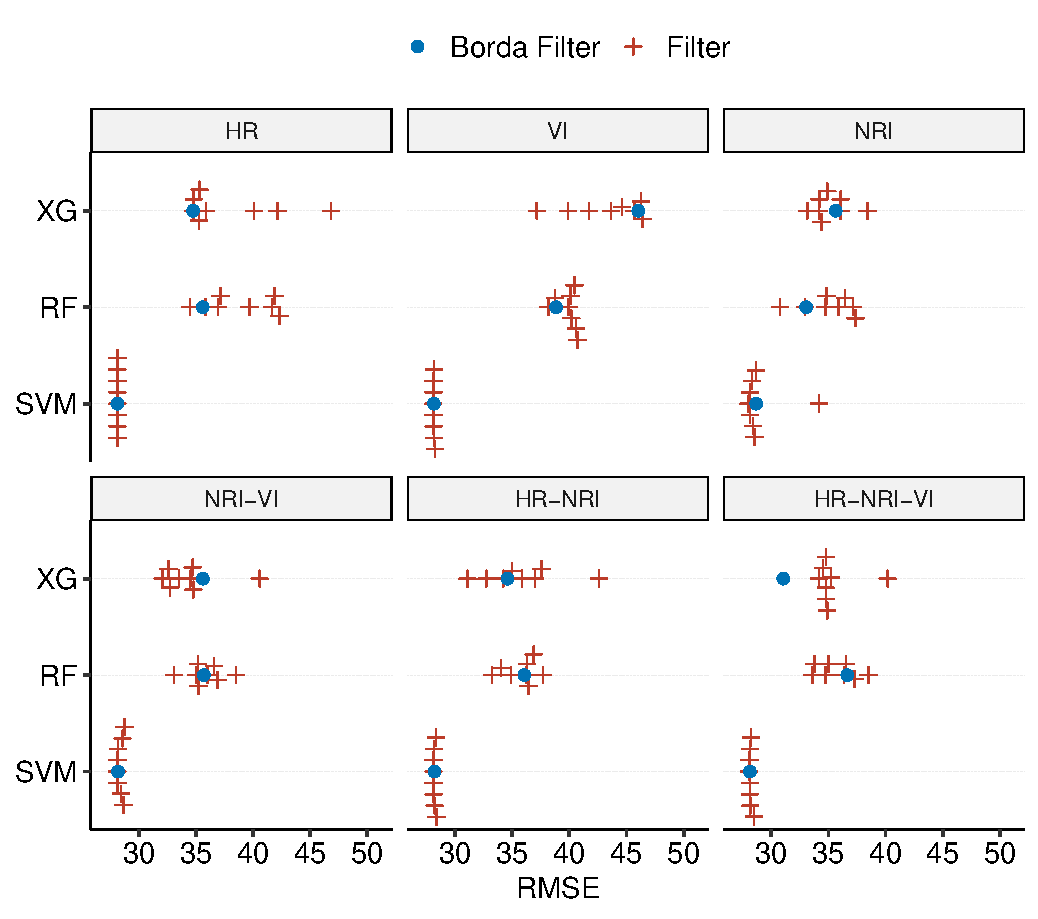
\includegraphics[width=0.48\textwidth] {filter-effect-all-vs-borda-filter-1.pdf}
		\caption{Model performances in RMSE when using the Borda filter method compared to all other filters for each learner across all tasks.}\label{fig:filter-effects-borda}
	\end{center}
\end{figure}

\subsection{Variable importance}

\subsubsection{Permutation-based Variable Importance}

% Variable Importance
% - VI: Vogelmann indices are best
% - All: Clustering around the red edge (700 - 750 nm)
% - Overall highest: 1.7 RMSE decrease - not that much

The most important features of each dataset showed an average decrease in RMSE of 1.57 (HR, B69) and 1.79 (VI, Vogelmann2) (\autoref{fig:fi-permut-vi-hr}).
For both datasets most features among the ten most important ones cluster around a wavelength range of 700 nm - 750 nm (the so called "red-edge").
For feature set HR four features in the infrared region (920 nm - 1000 nm) were identified by the model to be most important (causing a mean decrease in RMSE of around one percentage point).
Overall, most features show only a small importance with average decreases in RMSE below 0.5.

% permutation based var imp for datasets HR and VI
\begin{figure} [t!]
	\centering
	\begin{center}
		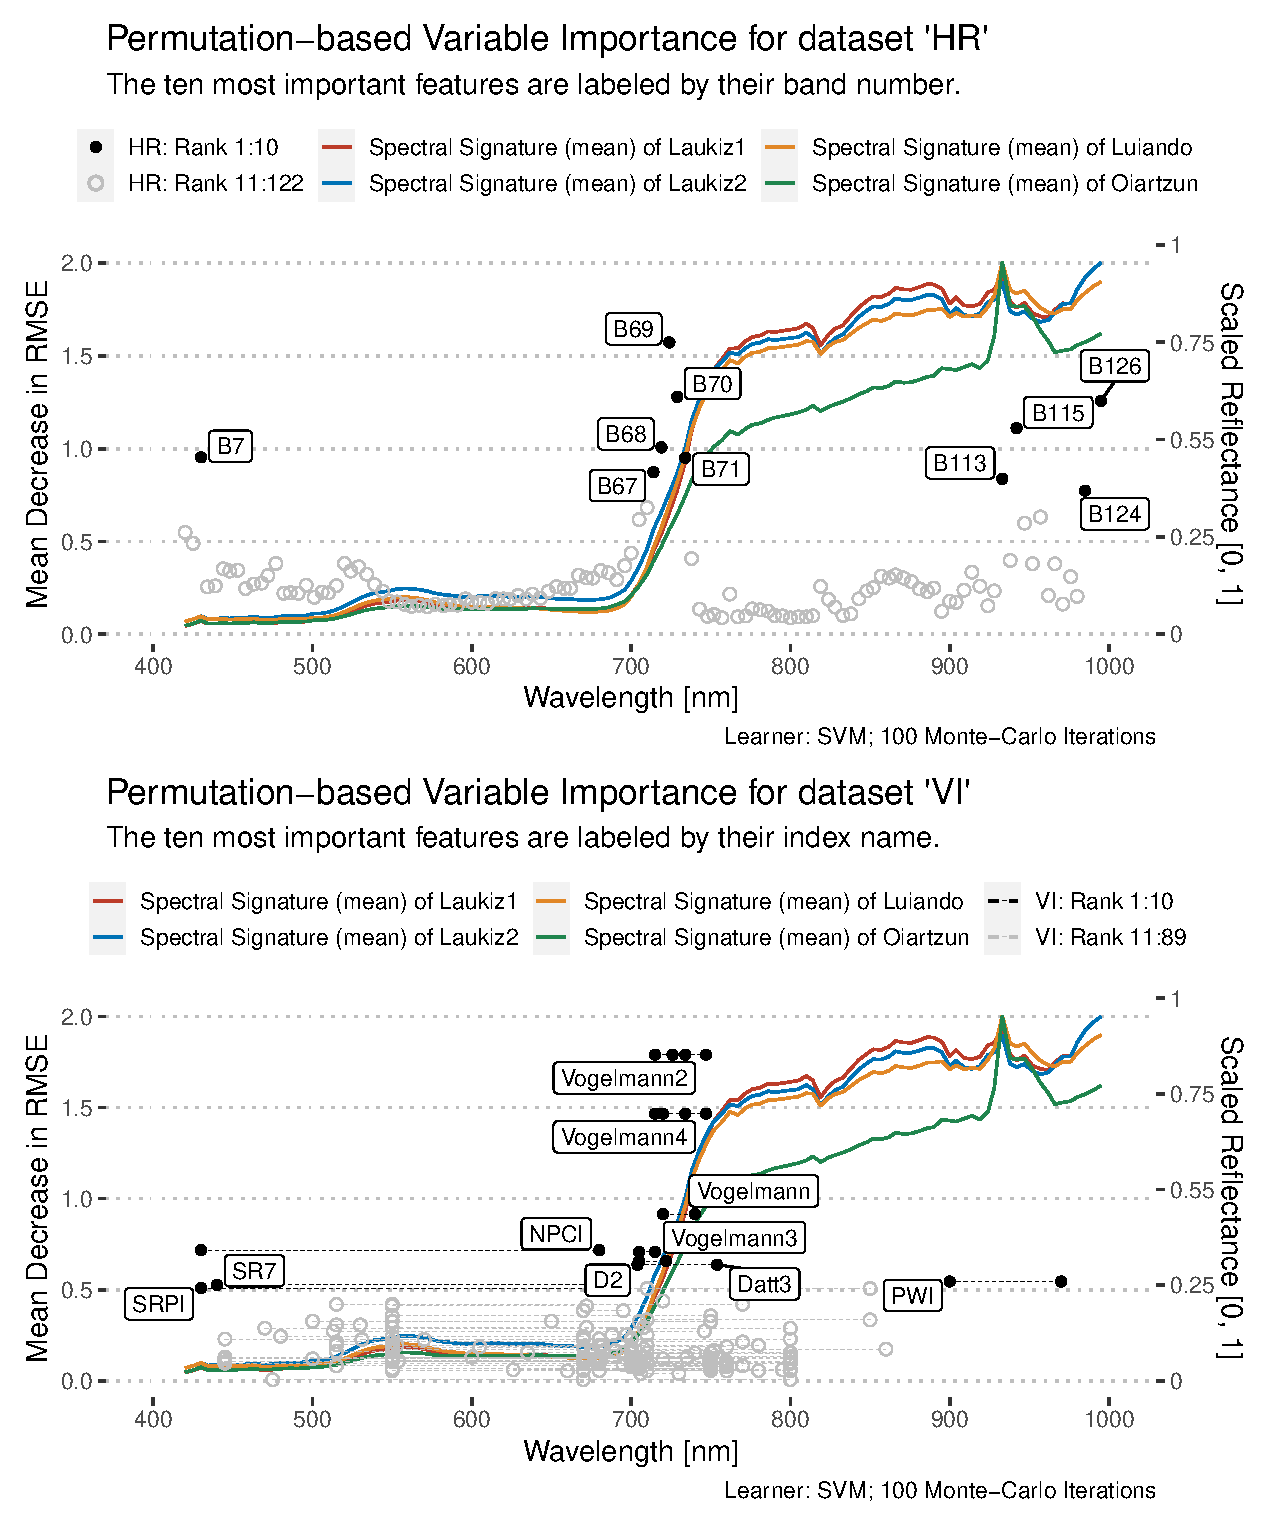
\includegraphics[width=0.48\textwidth] {fi-permut-vi-hr-1.pdf}
		\caption{Variable importance for feature sets HR and VI: Mean decrease in RMSE for one-hundred feature permutations using the SVM learner. The wavelength range on the x-axis matches the range of the hyperspectral sensor (400 nm - 1000 nm). For each dataset, the ten most important features were highlighted as black dots and labeled by name. Grey dots represent features from importance rank 11 to last. The spectral signature (mean) of each plot was added as a reference on a normalized reflectance scale [0, 1] (secondary y-axis). VI features were decomposed into their individual formula parts; all instances being connected via dashed lines. Each VI feature is composed out of at least two instances.}\label{fig:fi-permut-vi-hr}
	\end{center}
\end{figure}

\section{Discussion}

\subsection{Derivation of Indices}

\noindent The decision to use a buffer of 2 m to generate the index value for each observation has to be seen critical.
Due to the reported geometric offset of up to 1 m for the hyperspectral data, the possibility of assigning a wrong pixel value to a tree observation would be high.
Using a buffer of more than 2 meters increases the probability of including information from other trees into the pixel value, blurring the actual value of the tree observation.
In our view using a buffer of 2 m is a good compromise between both worlds.
In addition, a side-analysis showed that some trees would be assigned missing values when relying on a single pixel.
This then would result in the removal of that particular tree which we wanted to avoid.
Even though we provide no results showing the influence of multiple buffer values on the extraction, we hypothesize that the relationships between features would not change substantially, leading to the almost identical model results.

Another critical point is that the exact number of contributing pixels to the final index value of an observation cannot be determined as it depends on the location of the tree within the pixel grid.
According to the extract function of the \texttt{raster} package, a pixel is included if the buffer of the point observation hits the centroid of the respective pixel, not just any part of it.
As the buffer is circular, determining the total number of contributing pixels for each tree depends on the exact location of a tree within the pixel grid.
Next, if a tree observation is located at the border of the plot, some directions of the buffer will contain no values and the subsequent index value will be calculated using less pixels than if the tree observation is located in the middle of the plot.
The magnitude of uncertainty introduced by these facts cannot be quantified.
However, we assume these to be of minor importance for the subsequent model fitting step.

\subsection{Performance vs.\ plot characteristics}
\label{subsec:perf-plot-char}

\noindent The high differences in RMSE observed for the fold performances (\autoref{tab:svm-single-fold-perf}) are a result of model overfitting.
An RMSE of 54.26 indicates a complete failure of the model in the prediction stage for this plot (Laukiz2).
Laukiz2 differs highly in the distribution of the response variable defoliation compared to all other plots (\autoref{fig:defol-distr}).
The model overfitted on learning relationships related to medium-high defoliation values but missed out on low defoliation values.
In cases when Laukiz2 is in the training set, the model is able to half the error and even reduce it down to a value of 9 RMSE in the case of Luiando.

\subsection{Predictive Performance}
The best aggregated performance of this study (SVM + Carscore filter, 27.98 RMSE) has to be seen in the light of model overfitting (see \autoref{subsec:perf-plot-char}).
Leaving out the performance on Laukiz2 when aggregating results, the mean RMSE would be 19.
However, leaving out a single plot would also change the prediction results for the other plots because the observations from Laukiz2 would not be available for model training.
With the clear presence of model overfitting in this study it can be postulated that more training data representing all health stages of a plot is needed.
A model can only make robust predictions if it has learned relationships across the whole range of the response.
Hence, care should be taken when making statements about the overall performance of the fitted models of this study due to their high variance when predicting.
However, when inspecting the fold level performances, one can say that the model does a decent job predicting defoliation ranging from 50\% to 100\% but fails for 0\% - 50\%.
This applies to all learners of this study.

\subsubsection{Algorithm differences}
An interesting find is the strength of the SVM algorithm when comparing its predictive performance to its competitors (\autoref{tab:best-learner-perf}).

FIXME: Add refs
There were few environmental modeling studies only in recent years in which SVM outperformed other models that clearly.
The absolute difference of around three percentage points is also worth noting:
We could not find a study in which SVM came out as the best model in such clear way.
All of these statements are based on the assumption that a proper hyperparameter tuning was conducted for all models (which we also claim for ourselves in this study).

We were a bit surprised about the performances of the penalized methods Lasso and Ridge.
The former was not able to achieve an error below 45.96 RMSE across any dataset while Ridge came at least somewhat close to RF and XGBoost for some feature sets.
However, there were also three instances (VI, NRI-VI, HR-NRI-VI) for which the error of the fitted Ridge model was out of bounds.
We cannot preclude possible mistakes on our side when optimizing the penalization terms of the penalized learners.

FIXME: Talk about L1 and L2 model performance

\subsubsection{Feature set differences}
One objective which this study aimed to answer was whether expert-based or data-driven feature engineering has a positive influence on model performance.
With respect to \autoref{fig:perf-result} one can say that overall the different feature sets did not result in substantial changes in performance.
RF and XGBoost showed a somewhat surprising decrease in performance of about six percentage points on task VI compared to all others.
We have no explanation for this specific result, especially because the SVM does not show this difference.

FIXME: Talk about L1 and L2 models -> there we have quite some differences!

\subsection{Feature selection methods}

% - Effect varies across learners -> suggest to use FS even on feature sets with p < 100?
The usefulness of filters in this study was apparent across all feature sets, even when $p$ was rather small (HR).
Even though the effect of feature selection methods varied across algorithms, small to substantial improvement in predictive performance were achieved in almost all cases.
No optimal algorithm/filter/dataset setting was observed in this study, leading to the conclusion that one needs to try out various combinations of such to find the best performing one.

% - Ensemble FS shows no advantage to simple methods -> maybe to less features, features too correlated? check diff between effect on NRI and VI
We have no explanation why the Borda ensemble method used in this study did not score better than the average performance of other filter methods.
Ensemble methods shine in complicated scenarios when simple filter methods face problems due to their focus on certain areas of features.
We assume that the datasets used in this study were not complex enough to bring up these problems for simple features.
Therefore it makes sense that, due to its averaging nature, the Borda filter scored average results across all instances.
However, this cannot be known upfront and we believe that an ensemble filter should be part of every filter portfolio when doing filter-based feature selection.

% - PCA shows similar performance but probably requires tuning of main components -> check runtime!
The PCA approach did neither show the best or worst result in the lineup.
It shines in terms of runtime since it reduces the amount of features highly.
However, it also removes the option for a post-analysis of feature importance by squashing predictors into principal components and users need to decided upfront what they value more.
Since filters are only calculated once due to caching, the runtime advantage might in fact be negligible in practice.

\subsubsection{Linking feature importance to spectral characteristics}

Not surprisingly the most important features for both HR and VI datasets were identified around the red edge of the spectra, specifically in the range of 700 nm to 750 nm.

FIXME: Add ref
This area has the highest ability to distinguish between reflectances related to a high density / high healthiness of vegetation and its opposite.
It is also worth mentioning that four out of ten of the most important features of dataset HR lie between 920 nm and 1000 nm.
Looking at the spectral curves of the plots, we can observe quite some variance in this area, especially for Oiartzun, which might explain why these features were considered as important by the model.

\subsection{Comparison to other studies}
% - no environmental studies use filter methods, some use FFS
% - only few studies analyze defoliation
% - most FS is done in bioinformatics

\noindent Most other studies analyzing defoliation operated on the plot rather than the tree level.
This is due to the low spatial resolution of used satellite products which served as the input data, making a tree-level study infeasible \cite{townsend2012, debeurs2008, rengarajan2016}.

Studies focusing on tree-level defoliation used ground-level methods such as \ac{ALS} or \ac{LiDAR}\cite{meng2018, kalin2019}.
\cite{meng2018} used \ac{OLS} regression methods while\cite{kalin2019} retrieved information out of ground-level RGB photos using \ac{CNN}.
Both study designs are substantially different compared to the setup of this work.
In addition, no spatial \ac{CV} or \ac{FS} was used.
\cite{goodbody2018} used a \ac{PLS} model with high-resolution \ac{DAP} to predict cumulative defoliation caused by the spruce budworm.
Study results indicated that spectral metrics were found to be most helpful for the model.
Incorporating such metrics (both spectral and structural) could be a possible enhancement for future works.

\cite{shendryk2016, ludwig2019} are studies which are more similar in their methodology but focus on a different response variable (woody cover).
\cite{shendryk2016} used machine learning with \ac{ALS} data to study dieback of trees for eucalyptus forests.
A grid-search was used for hyperparameter tuning and \ac{FFS} for variable selection.
\cite{ludwig2019} analyzed woody cover in South Africa using spatial \ac{CV} and \ac{FS} approach \cite{meyer2018} with a Random Forest classifier.

In summary, we could not find studies using filter methods for \ac{FS} or \ac{NRI} indices in their work with a relation to forest health.
Most studies used only one algorithm (usually Random Forest) without (strong) arguments why this particular one has been selected or why only one model was used.
This is not surprising: Most environmental/ecological datasets are not high-dimensional.
In contrast, the number of predictors if often monadic and issues related to correlations are solved manually instead of relying on an automated approach.
The bioinformatics field faces high-dimensional feature sets more often.
Hence more studies using (filter-based) feature-selection approaches can be found for this field \cite{guo2019, radovic2017}.
If a field only rarely faces high-dimensional dataset issues the motivation and expertise of using advanced methods to solve such are rather low.
We hope that this work can give some guidance and serve as a starting point for tackling high-dimensional problems in environmental modeling.

\section{Outlook and conclusion}
This study analyzed defoliation at trees in north Spain by using hyperspectral data as input for machine learning models making heavy use of filter-based feature selection methods.
It was shown that substantial differences in performance can occur depending on which feature selection methods and machine learning algorithms are combined.
SVM showed the most robust behavior across all highly-correlated datasets and was able to predict the response variable of this study substantially better than other methods.

% RQ3: How are feature-selection methods influencing the predictive performance of the models?
Filter methods showed their ability to improve predictive performance for datasets with many features.
Ensemble filter methods did not show a substantial improvement over legacy filter methods.

% RQ2: Does combining feature sets have an substantial effect on predictive performance?
% RQ1: Do different environmental feature sets show differences in performance when modeling defoliation at trees?
FIXME: "derivated" is not a real word?
Creating feature sets composed out of derivated features did not help.
In contrast, dataset VI showed a substantial worse performance than the dataset with the original features (HR).
Combining feature sets did not show a substantial improvement on predictive performance.

% RQ4: Which features are most important for the models and how can these be interpreted in an ecological context?
Features along the red-edge wavelength region were most important for models to achieve good predictions.
With respect to dedicated vegetation indices, the "Vogelmann" index with all of its versions was seen as the most important index for the tested SVM algorithm.

% What about the general potential of analyzing defol with hyperspectral data?
The potential of predicting defoliation for single trees with the given toolset of this study was rather limited, seen on the average error of 27\%. 
However, with better training data covering more variety of the response variable, performance could be highly improved in future studies.

\appendices{}

\section{SVM ALE plots for task HR}

\begin{figure} [ht]
	\begin{center}
		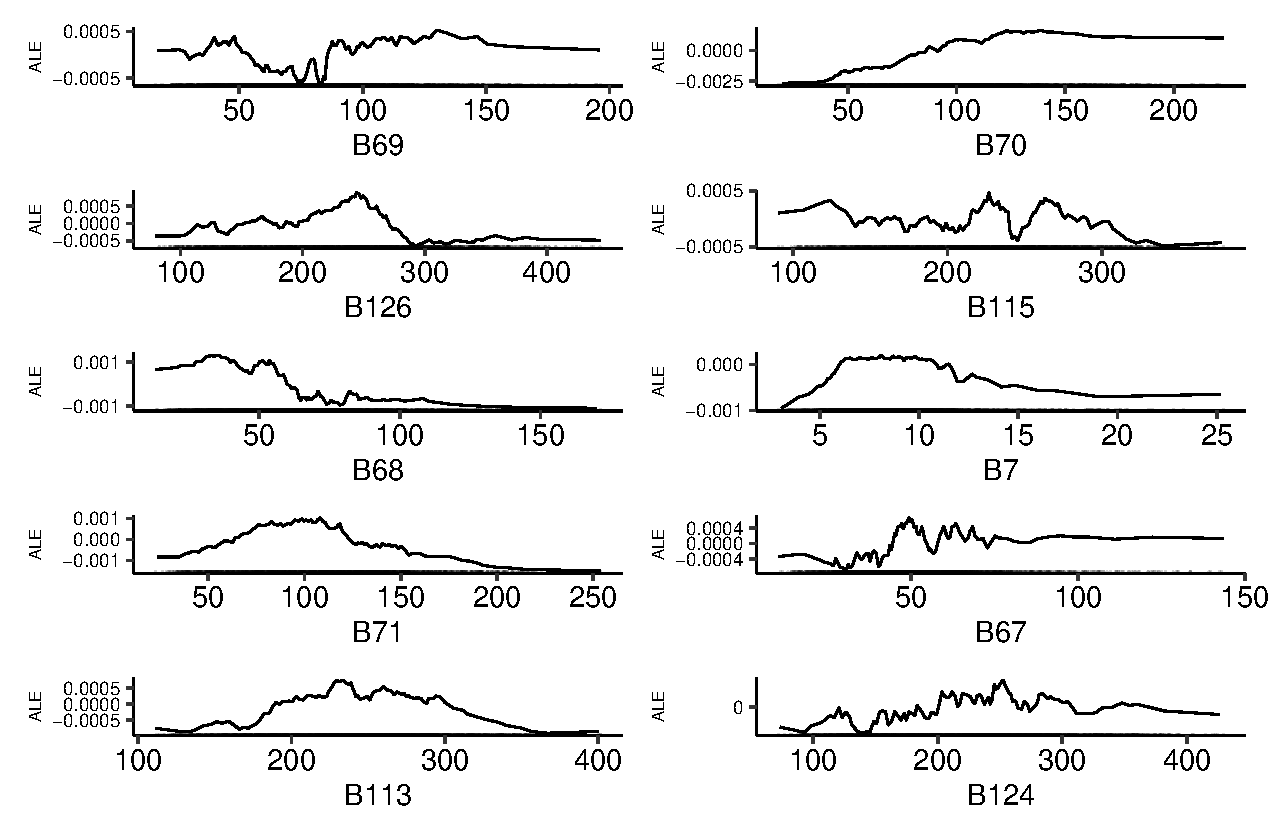
\includegraphics[width=0.48\textwidth] {fi-hr-ale-1.pdf}
		\caption{ALE plots on dataset HR of SVM learner. Subset showing the ten most important features according to the permutation-based variable importance. The y-axis shows the deviation to the mean prediction for each feature, with the mean prediction being centered at zero.}\label{fig:fi-hr-ale}
	\end{center}
\end{figure}

\section{SVM ALE plots for task VI}

\begin{figure} [ht]
	\begin{center}
		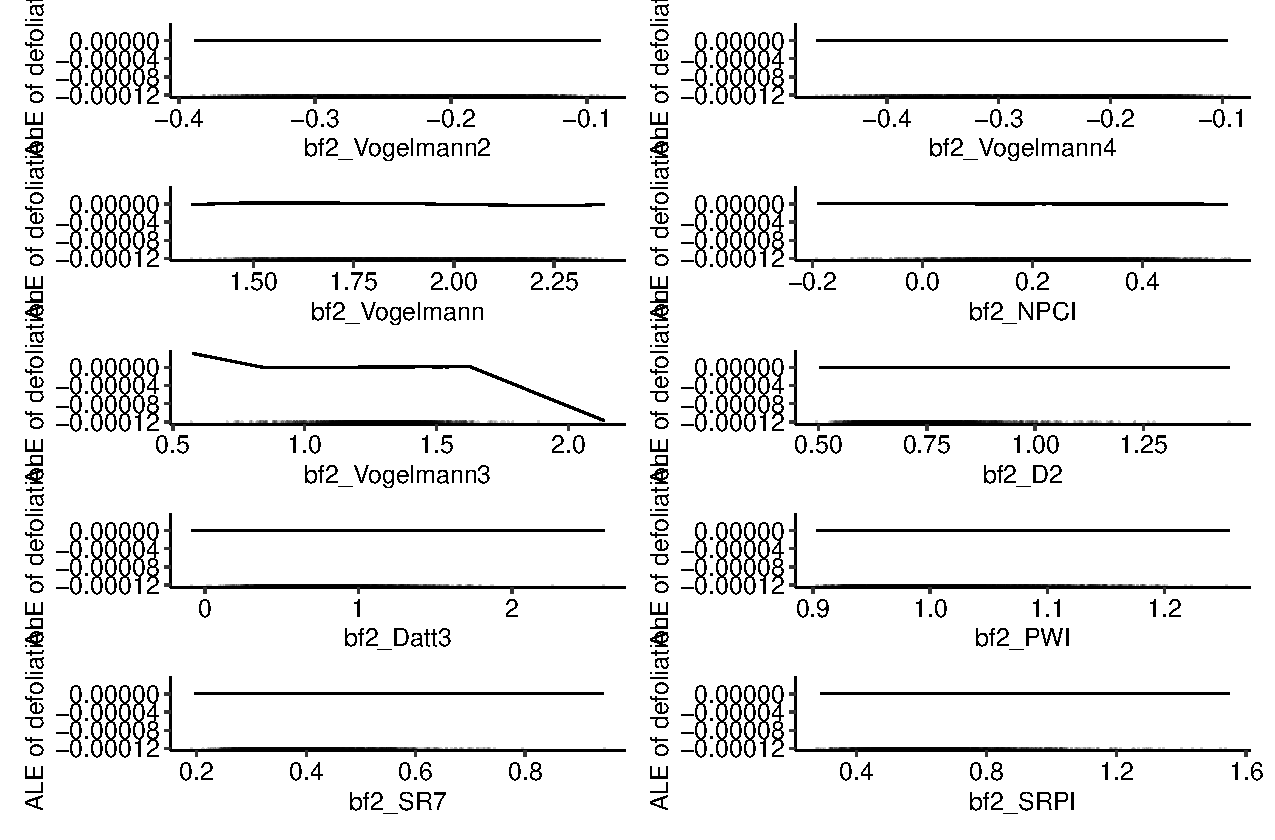
\includegraphics[width=0.48\textwidth] {fi-vi-ale-1.pdf}
		\caption{ALE plots on dataset VI of SVM learner. Subset showing the ten most important features according to the permutation-based variable importance. The y-axis shows the deviation to the mean prediction for each feature, with the mean prediction being centered at zero.}\label{fig:fi-vi-ale}
	\end{center}
\end{figure}

\section{Correlation among filter methods}

\pagebreak

\begin{figure} [ht]
	\begin{center}
		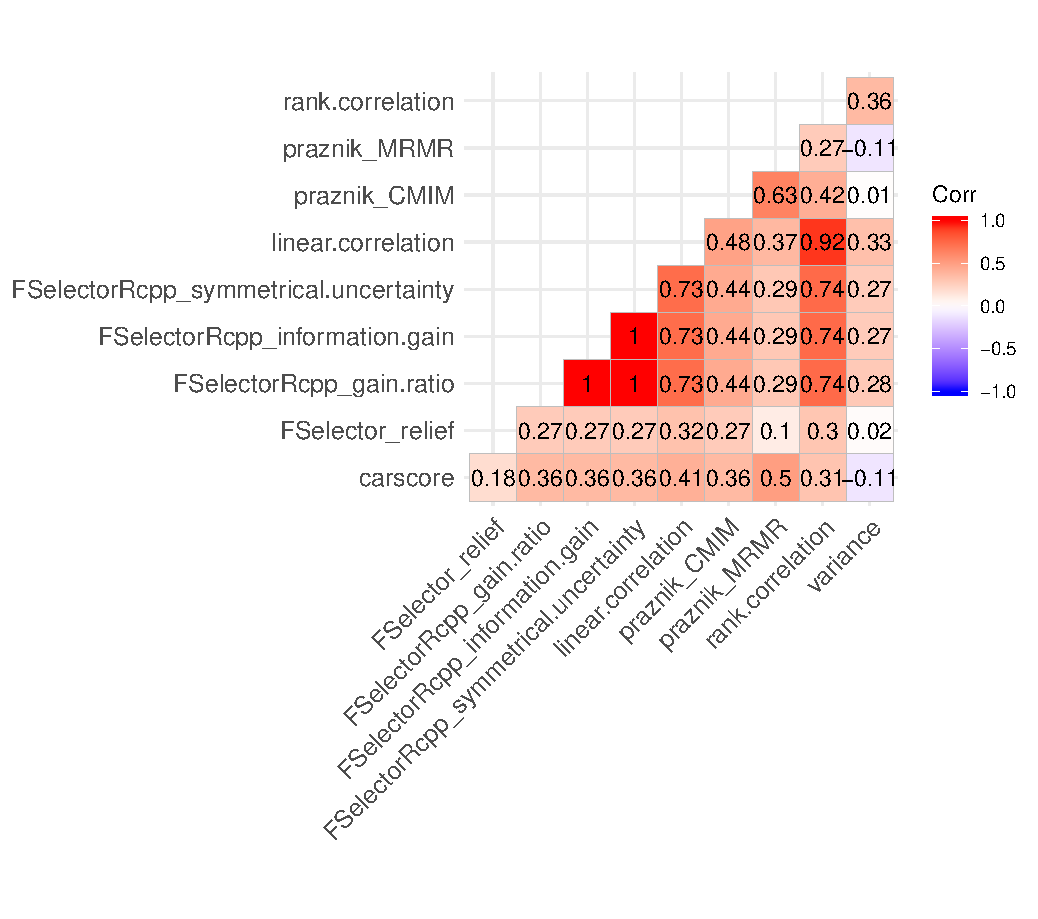
\includegraphics[width=0.48\textwidth] {correlation-filter-nri-1.pdf}
		\caption{Spearman correlation of filter rankings between various filter methods. Results of the NRI feature set are shown.}\label{fig:correlation-filters}
	\end{center}
\end{figure}

\section{Effect of different \texorpdfstring{\(n_{bins}\)}{nbins} values on filter 'information gain'}

\begin{figure} [ht]
	\begin{center}
		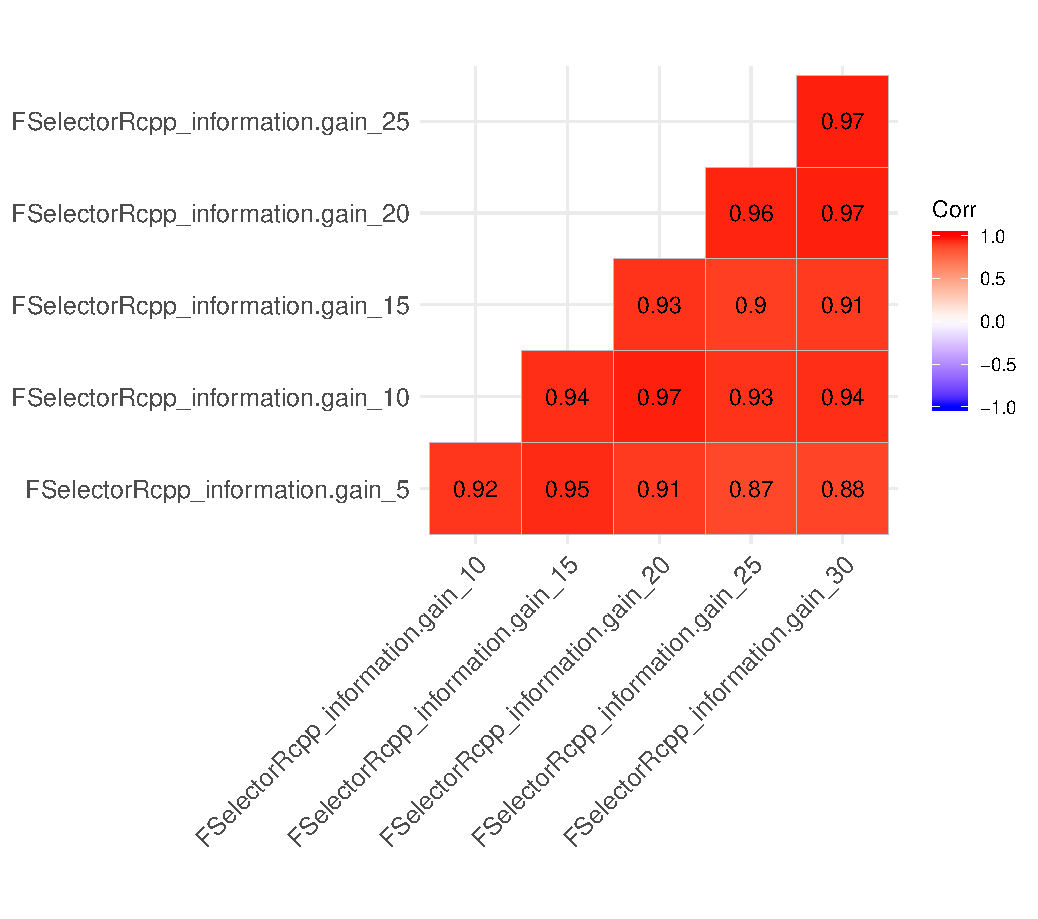
\includegraphics[width=0.48\textwidth] {correlation-nbins-1.pdf}
		\caption{Spearman correlation of filter information gain using different \texttt{\(n_{bins}\)} values for discretization of the numeric response.}\label{fig:correlation-nbins}
	\end{center}
\end{figure}

\pagebreak

\bibliographystyle{IEEEtran}
\bibliography{Biblio}

\section*{References}

\end{document}

